% CREDITS:
% Comprehensive exam template for ECE Ph.D. students at Queen's University. by Jefferson Silveira
\documentclass[a4paper,10pt]{article}
\usepackage[left=25mm,top=25mm,right=25mm,bottom=25mm]{geometry}
\usepackage{etoolbox} %required for cover page
\usepackage{booktabs}
\usepackage[T1]{fontenc}
\usepackage[utf8]{inputenc}
\usepackage{lmodern}
\usepackage{bm}
\usepackage{graphicx}
\usepackage{subcaption}
\usepackage{amsmath}
\usepackage{amsfonts}
\usepackage{mathtools}
\usepackage[dvipsnames]{xcolor}
\usepackage{float}
\usepackage{hyperref}
\usepackage[capitalise]{cleveref}
\usepackage{enumitem}
\usepackage{amssymb}
\usepackage{comment}
\usepackage{multirow}

\usepackage[italian]{babel}
% "text" in the source is printed with the right opening and closing quotes
\usepackage[autostyle=false, style=english]{csquotes}
\MakeOuterQuote{"}
\frenchspacing % same space after a full stop as between words (Italian style)

\hypersetup{
    colorlinks,
    linkcolor={black},
    citecolor={blue!50!black},
    urlcolor={blue!80!black}
}

\linespread{1.1}

\graphicspath{{figures/}}

% ------------------- important:

\begin{document}

\pagenumbering{gobble} % remove page numbers (and reset to 1)

% -------------------------------- Front page
\newcommand{\docente}{Maurizio Zamboni}

\newcommand{\data}{Gennaio 2026} % CHANGE HERE

\newcommand{\subtitle}{Laboratorio di Sistemi Digitali Integrati}
\newcommand{\titolo}{Esercitazione finale di progetto sulle architetture integrate: Operazione San Silvestro}
\title{Relazione}
\newcommand{\curso}{Corso di Laurea in Ingegneria Elettronica (LM-29)}

% -------------------------------- Front content
\begin{center}\leavevmode
    \normalfont
    
\includegraphics[width=0.75\columnwidth]{img/polito_logo.png}
    \vskip 1cm
    {\large \curso}
    \vskip 1cm
    \rule{\linewidth}{0.2 mm}
    {\huge \bfseries \titolo \par}
    \vskip 1cm
    {\Large \bfseries \subtitle \par}

    \rule{\linewidth}{0.2 mm}\\[1.5 cm]

    \begin{minipage}[t]{0.55\textwidth}
    	\begin{flushleft} \large
    		\emph{Membri del gruppo}\\
            S307463 - Riccardo Moiso\\
            S358829 - Luca Magarotto
    	\end{flushleft}
    \end{minipage}
    \begin{minipage}[t]{0.35\textwidth}
        \begin{flushright} \large
        	{\emph{Docente}}\\
        	\ifdefempty{\docente}{}{\docente\\}
        \end{flushright}
    \end{minipage}
    \vfill
    {\normalsize \data\par}
\end{center}
\cleardoublepage

\tableofcontents
\newpage

\pagenumbering{arabic} % Arabic page numbers (and reset to 1)

% Sections
\section{Introduzione}
L’obiettivo di questo progetto è creare una fft a 16 campioni applicando l’algoritmo di Cooley-Tukey, che permette di semplificare e ridurre il numero delle operazioni necessarie. Date quindi le richieste e le limitazioni sui componenti da impiegare dovevamo ottenere le migliori performance possibili.
Si sono quindi sviluppate 2 modalità d’uso (descritte nella sottosezione \ref{subsec:modalità}): singola e continua. La seconda permette di aumentare il throughput a una solve ogni 6 colpi di clock.

\section{Data Flow Diagram}
\noindent Per Data Flow Diagram si intende uno schema in cui i blocchi rappresentano le varie operazioni, mentre le frecce descrivono il flusso dei dati. In questo caso, esso illustra come sono state distribuite le risorse, definite nella specifica, per unità di butterfly. Nel diagramma presentato di seguito, con un rettangolino nero si indica che il dato è salvato in un certo registro, l'asse verticale è quello temporale e presenta fino a dodici colpi di clock.

\begin{figure}[H]
      \centering
      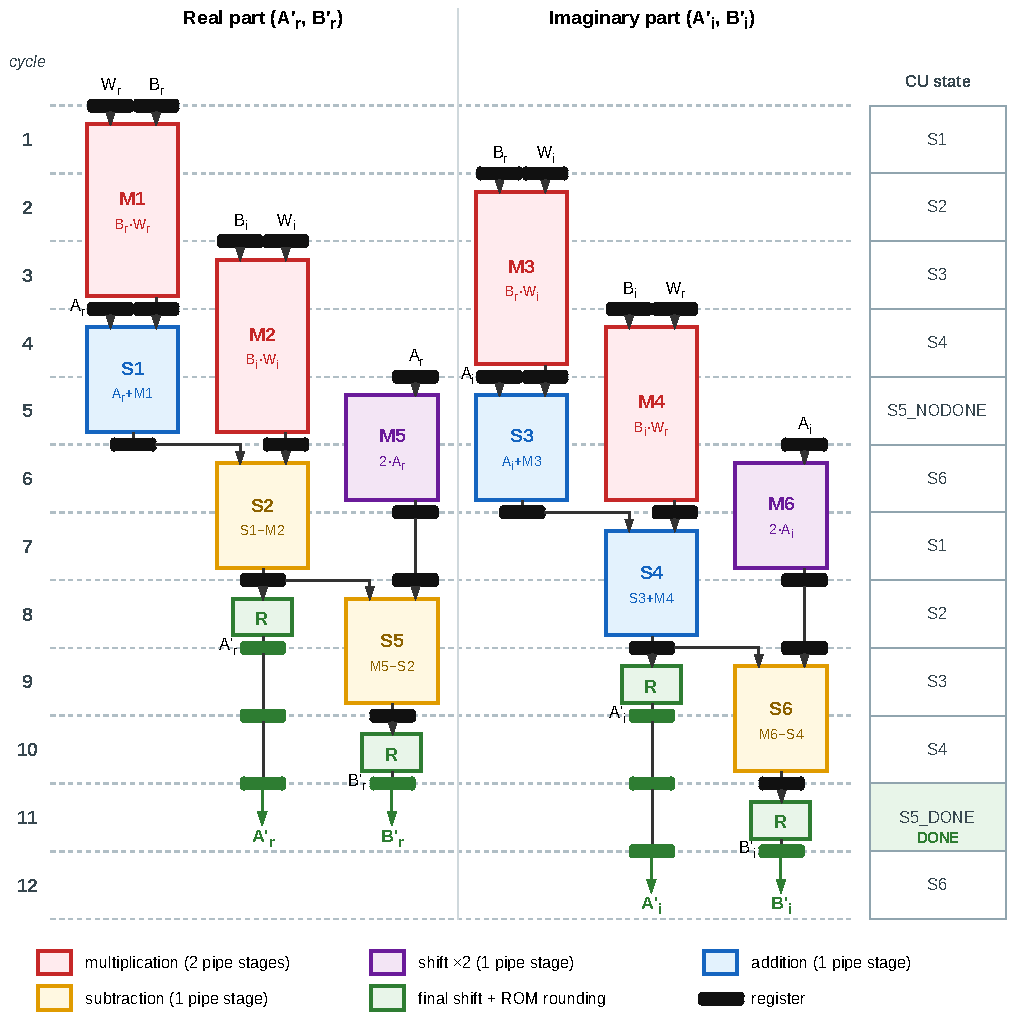
\includegraphics[width=1\textwidth]{fig01_dfd_butterfly}
      \caption{Data Flow Diagram dell'unità butterfly}
\end{figure} 

\noindent L'algoritmo da implementare prevede che l'unità compia le seguenti operazioni:
\begin{align*}
    A' &= A + B \cdot W^k \\
    B' &= A - B \cdot W^{(k+N/2)}
\end{align*}

\noindent dove A', B', A, B e i $W$ sono in generale dei numeri complessi. 
\noindent Da specifiche, all'interno di una singola butterfly, si hanno a disposizione un solo sommatore e un solo sottrattore, entrambi con uno stadio di pipe e un unico blocco che, a seconda di un segnale di controllo, può compiere una moltiplicazione caratterizzata da due stadi di pipe, oppure uno shift aritmetico verso sinistra dell'ingresso di una locazione (con uno stadio di pipe). Tutti questi blocchi svolgono operazioni su numeri reali. Perciò, è necessario scomporre le variabili nella loro parte Reale ($r$) e Immaginaria ($i$), e lavorare su queste. Al fine di ottenere i 4 risultati voluti $A'_r$,  $B'_r$, $A'_i$, $B'_i$ (ovvero le parti reali e immaginarie degli ingressi e delle uscite), è necessario svolgere 4 moltiplicazioni ($M_1$, $M_2$, $M_3$ e $M_4$), 2 shift aritmetici ($M_5$ e $M_6$), 3 somme ($S_1$,$S_3$ e $S_4$) e 3 sottrazioni ($S_2$, $S_5$ e $S_6$).

\begin{comment}
\begin{itemize}
    \item \textbf{Prodotto Complesso} ($P = B \cdot W$):
    \begin{itemize}
        \item $P_r = B_r W_r - B_i W_i$
        \item $P_i = B_r W_i + B_i W_r$.
     Richiede quattro moltiplicazioni, una sottrazione e una somma.
    \end{itemize}
    
    \item \textbf{Somma/Sottrazione Butterfly}:
    \begin{itemize}
        \item $A'_r = A_r + P_r, \quad A'_i = A_i + P_i$
        \item $B'_r = A_r - P_r, \quad B'_i = A_i - P_i$. Richiede due somme e due sottrazioni.
    \end{itemize}
\end{itemize}
\end{comment}

\noindent Avendo a disposizione un solo moltiplicatore/shifter fisico, le operazioni che lo necessitano devono essere serializzate. Il diagramma mostra sei utilizzi di tale blocco per ciascuna esecuzione della butterfly, indicati come segue:

\begin{itemize}
    \item Ciclo 1: si inizia l'esecuzione del calcolo $M_1 = B_{r} \quad \cdot \quad W_{r}$
    \item Ciclo 2: si inizia l'esecuzione del calcolo $M_3 = B_{r} \quad \cdot \quad W_{i}$
    \item Ciclo 3: si inizia l'esecuzione del calcolo $M_2 = B_{i} \quad \cdot \quad W_{i}$
    \item Ciclo 4: si inizia l'esecuzione del calcolo $M_4 = B_{i} \quad \cdot \quad W_{r}$
    \item Ciclo 5: si opera su $A_{r}$, moltiplicandolo per un fattore 2 mediante uno shift verso sinistra, iniziando il calcolo di $M_5$
    \item Ciclo 6: si opera su $A_{i}$, moltiplicandolo per un fattore 2 mediante uno shift verso sinistra, iniziando il calcolo di $M_6$
\end{itemize}
Invece, di seguito, si presentano le operazioni effettuate dal sommatore e dal sottrattore e in quale colpo di clock esse iniziano ad essere eseguite, specificando che i risultati di $S_2$, $S_4$, $S_5$, e $S_6$, a seguito di un opportuno arrotondamento, corrispondono alle uscite volute della butterfly $A'_r$, $A'_i$, $B'_r$ e $B'_i$.
\begin{itemize}
    \item Ciclo 4: si esegue il calcolo $S_{1} \quad = \quad A_{r} \quad + \quad M_1$
    \item Ciclo 5: si esegue il calcolo $S_{3} \quad = \quad A_{i} \quad + \quad M_3$
    \item Ciclo 6: si esegue il calcolo $S_{2} \quad = \quad S_{1}\quad - \quad M_2  \quad (= A'_{r}\ )$
    \item Ciclo 7: si esegue il calcolo $S_{4} \quad = \quad S_{3} \quad + \quad M_4  \quad (= A'_{i}\ )$
    \item Ciclo 8: si esegue il calcolo $S_{5}\quad = \quad M_5 \quad - \quad S_{2}  \quad (= B'_{r}\ )$
    \item Ciclo 9: si esegue il calcolo $S_{6}\quad = \quad M_6 \quad - \quad S_{4}  \quad (= B'_{i}\ )$
\end{itemize}
 
\noindent Infine, i blocchi verdi presenti nel DFD corrispondono allo stadio di "rounding": sono collocati alla fine di ogni catena di calcolo per riportare i risultati a 24 bit prima di fornirli in uscita. Come indicato nelle specifiche, l'arrotondamento richiede un ulteriore ciclo di clock per generare il valore finale, poiché il risultato approssimato deve essere salvato in un registro.

\noindent Il Data Flow Diagram proposto è una soluzione che si avvicina maggiormente alla tipologia ASAP ("As Soon As Possible"), obbligata dalla possibilità di utilizzo di un singolo moltiplicatore e dalla richiesta di andare il più veloce possibile.
Inoltre, anche le altre operazioni avvengono tutte il prima possibile, poiché, appena sono disponibili tutti gli operandi, si inizia una nuova operazione.

\noindent Si evidenzia, inoltre, che, dal settimo colpo di clock, il moltiplicatore non deve più eseguire nuove operazioni della butterfly appena considerata e non è più necessario mantenere salvati gli ingressi: l'unità può quindi iniziare nuovamente con il prodotto $M_1$ del nuovo set di dati. Di conseguenza, la singola elaborazione degli ingressi da parte del PE impiega dodici colpi di clock per completare tutte le operazioni e fornire in uscita tutti i risultati, ma l'unità può ricevere in ingresso nuovi dati ogni sei cicli. Quanto descritto è ciò che accade nel caso in cui si utilizzi l'unità in modalità continua,  come descritto nelle sezioni successive.
\begin{figure}[H]
      \centering
      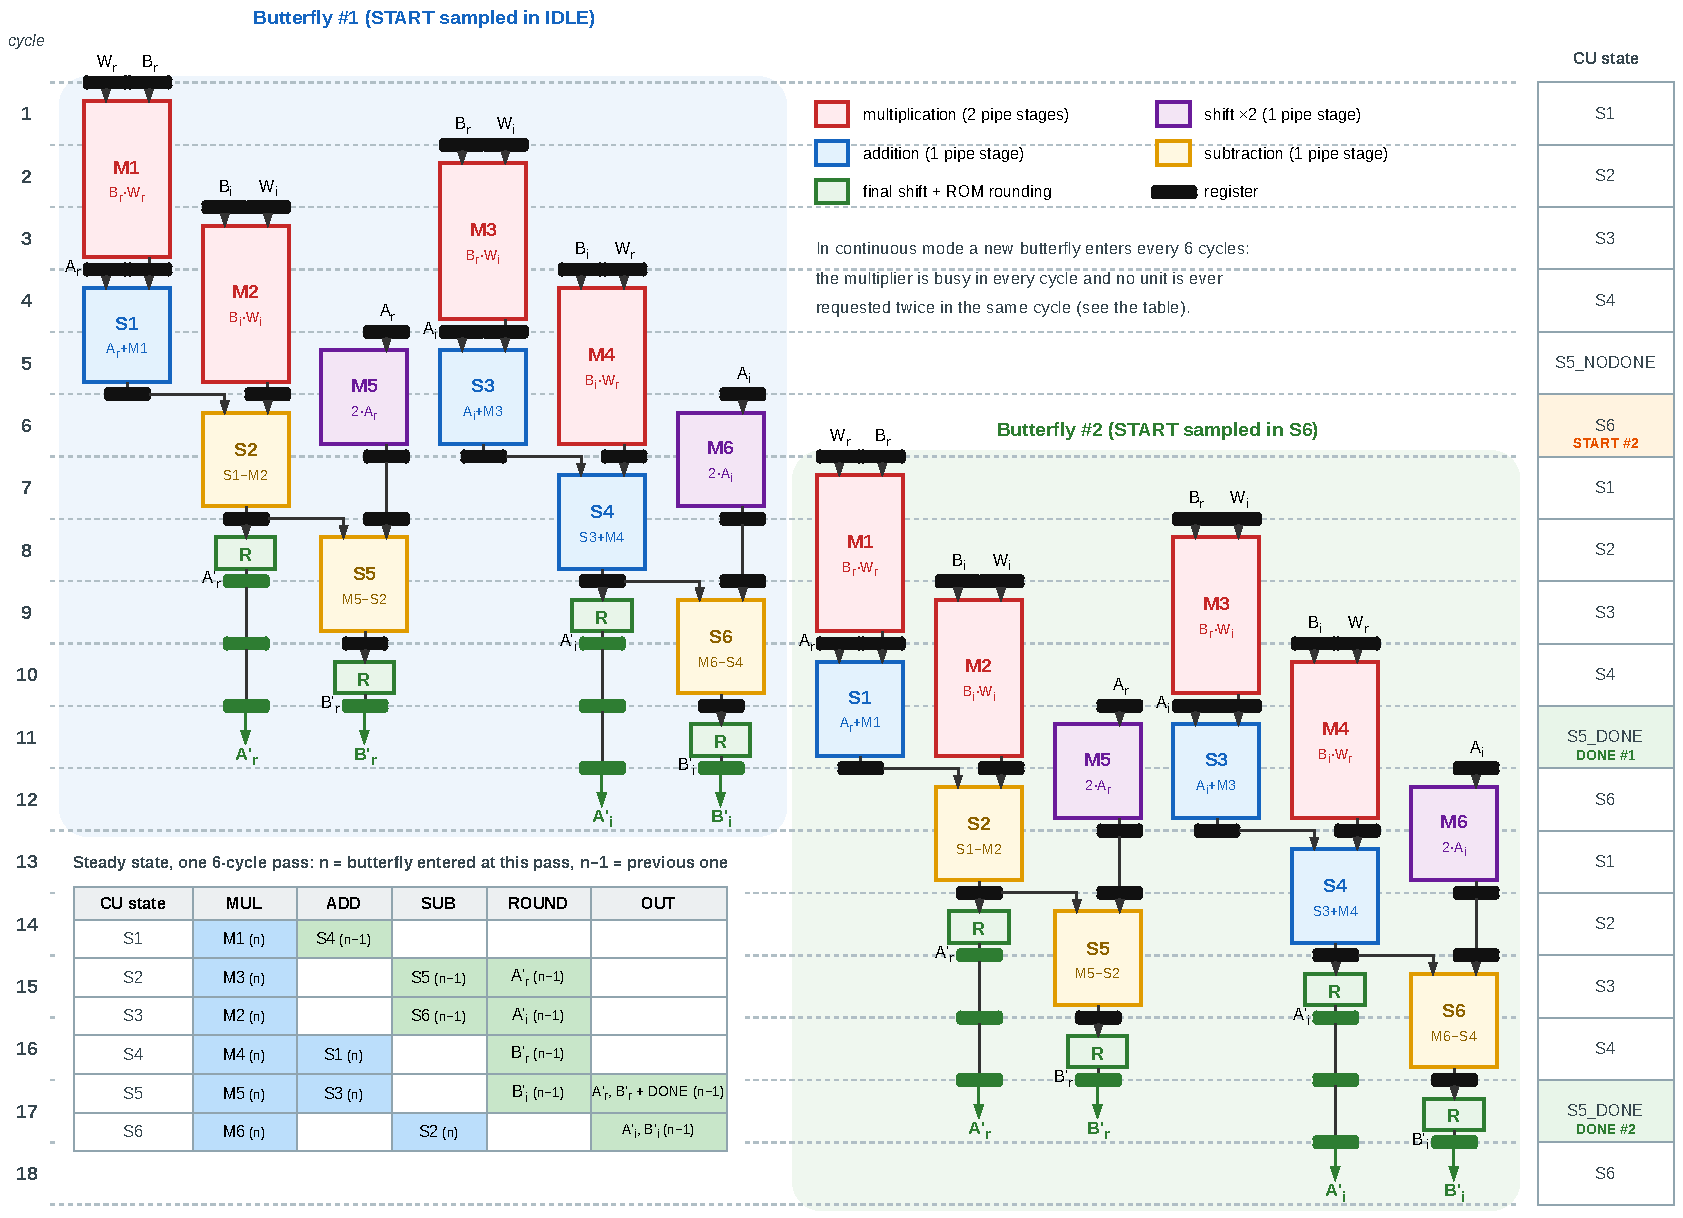
\includegraphics[width=1\textwidth]{fig02_dfd_continuous}
      \caption{Data Flow Diagram dell'unità butterfly in continua}
\end{figure}

\section{Tempo di vita delle variabili}

\noindent Il diagramma del tempo di vita delle variabili rappresenta graficamente l'occupazione dei registri e la durata di persistenza di ogni dato all'interno del datapath durante l'esecuzione dell'algoritmo, ossia da quando viene campionato fino a quando viene utilizzato per l'ultima volta da un operando. L'asse orizzontale indica i colpi di clock, quello verticale elenca i dati in ingresso, i prodotti, le somme algebriche intermedie ed i risultati finali; il colore di ogni casella indica il registro in cui il dato è salvato.

\noindent Le parti reali dei dati di input sono presenti già al primo ciclo, per poter alimentare la prima moltiplicazione, di seguito vengono fornite le parti immaginarie. Troviamo quindi i cicli spiegati precedentemente che si sovrappongono fra loro. Inoltre, si è deciso di rappresentare l’andamento nel tempo in più iterazioni della stessa Butterfly (indicate con \#1, \#2 e \#3), quando questa lavora in modalità continua, come si può facilmente notare dalle righe del diagramma riguardanti i dati in ingresso, dove la prima occupazione di \#2 e la prima di \#1 sono distanziate da 6 colpi di clk.

\noindent Si nota che, escludendo i valori in ingresso, il numero massimo di variabili che si osservano in un ciclo è pari a 5, come si vede, ad esempio, nel ciclo 11. Per tale ragione, per non scomodare il sistema di memorizzazione degli ingressi, si è scelto di introdurre nel datapath 5 registri dediti al salvataggio dei risultati intermedi e finali, come mostrato nella sezione successiva.

\begin{figure}[H]
      \centering
      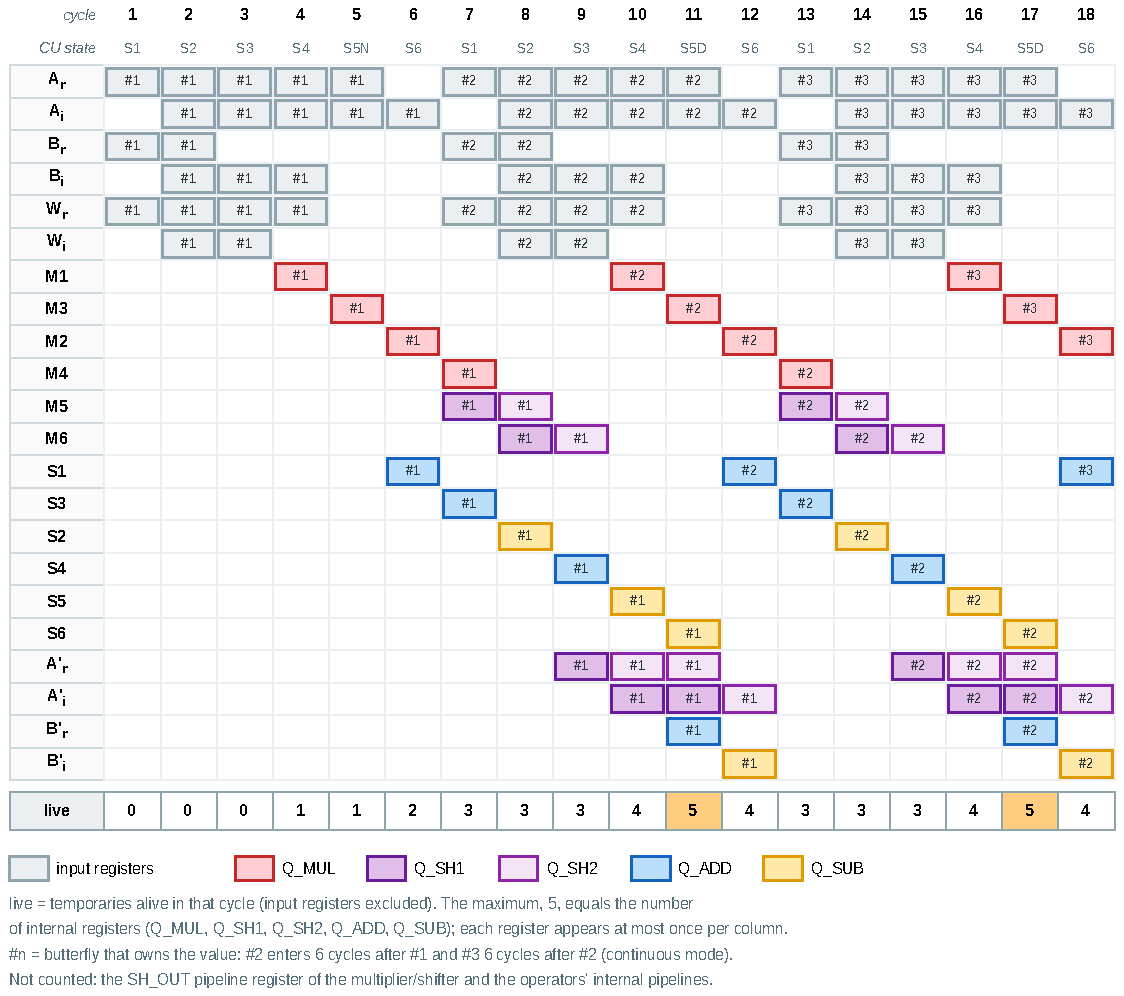
\includegraphics[width=1\textwidth]{fig11_variable_lifetime}
      \caption{Tempo di vita delle variabili}
\end{figure}

\section{Datapath}

\begin{figure}[H]
      \centering
      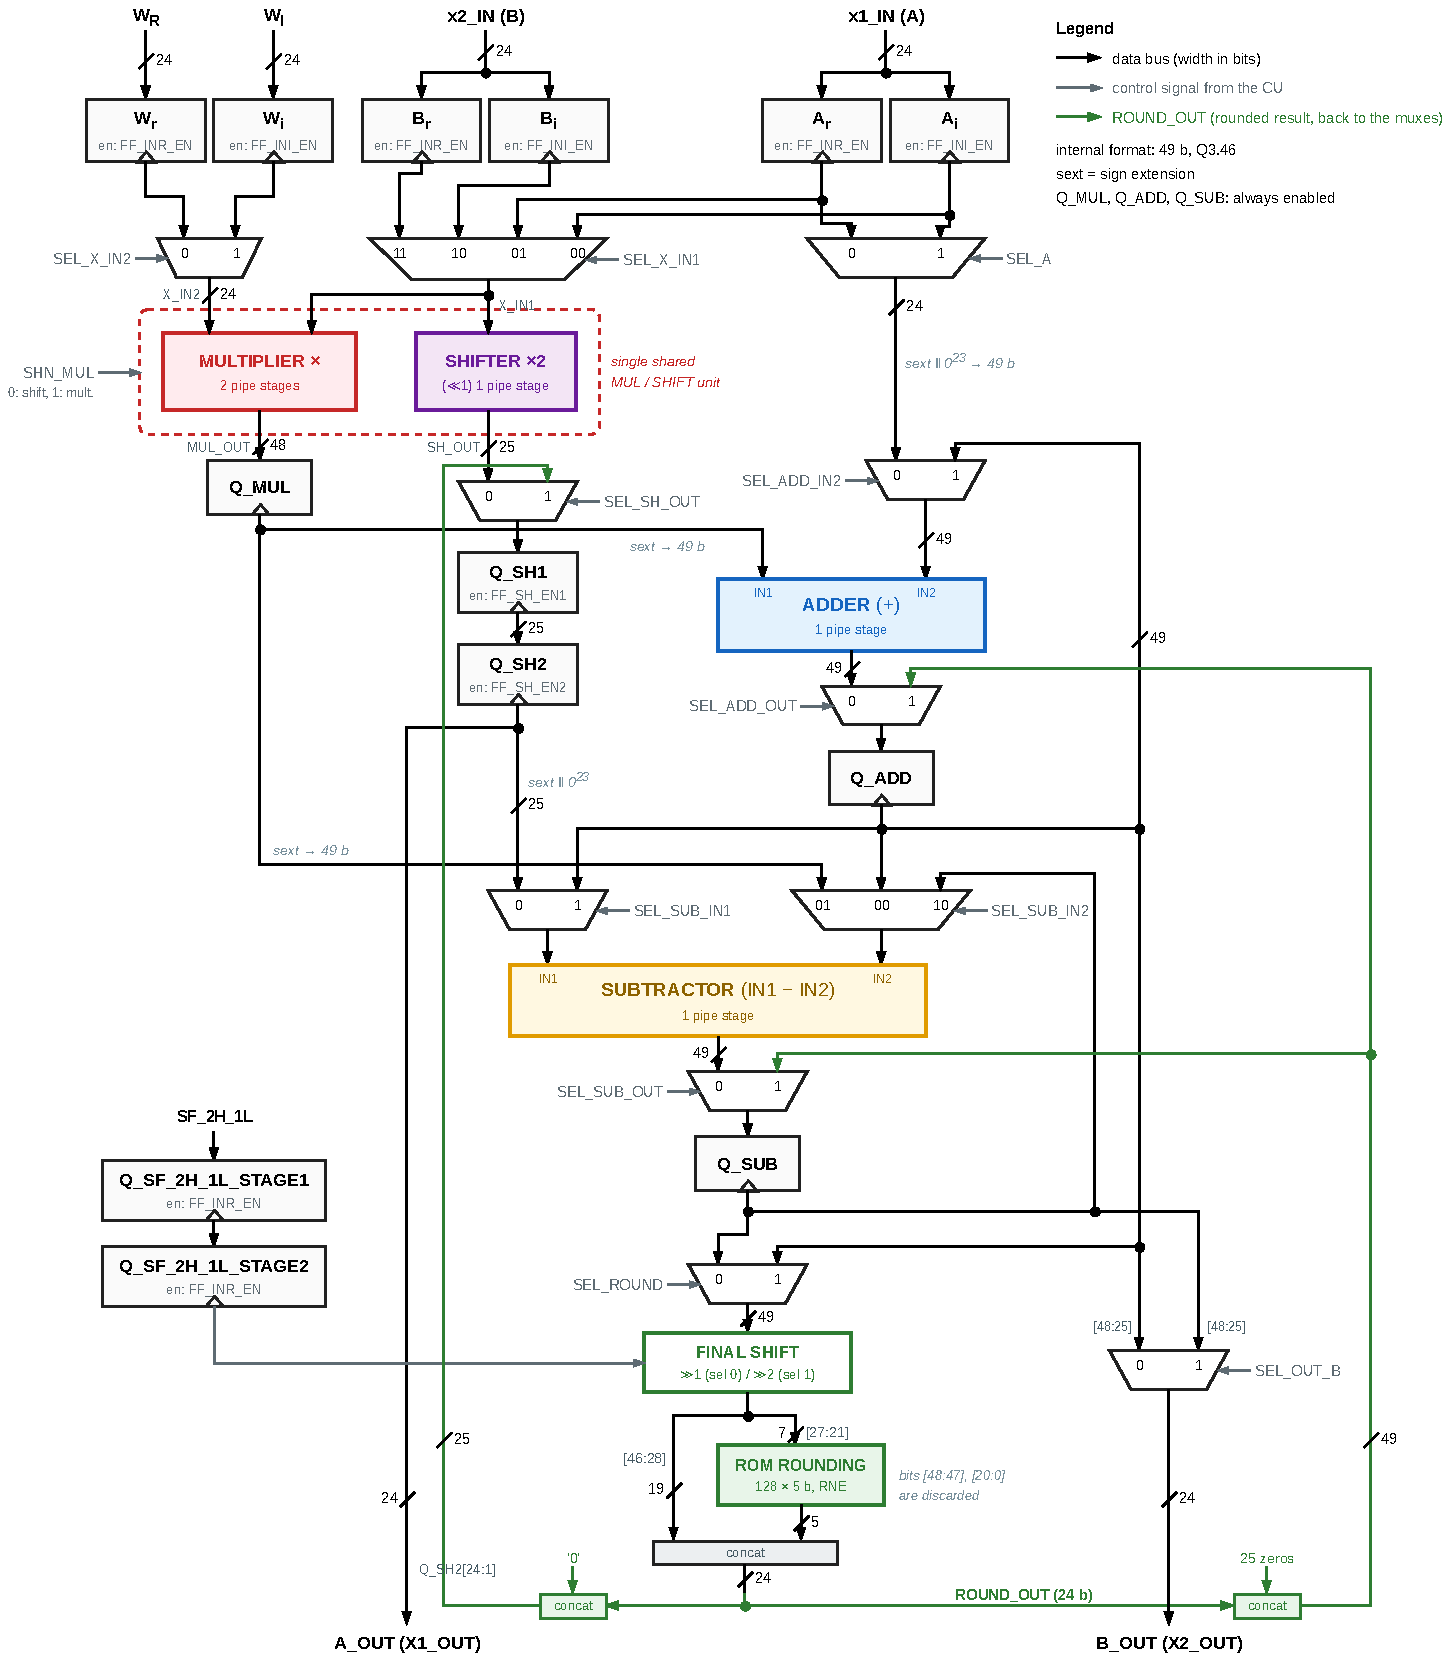
\includegraphics[width=1\textwidth]{fig03_datapath}
      \caption{Datapath dell'unità butterfly}
\end{figure} 

\noindent L'interfaccia in ingresso si occupa di acquisire i dati complessi di input A, B ed i coefficienti di rotazione W. Come richiesto dalle specifiche, per parallelizzare il caricamento dei valori, i bus di ingresso di A e B sono separati. Si introducono due registri per ogni parametro A, B, W, uno per la parte reale ed uno per la parte immaginaria. Essi sono abilitati da specifici segnali di controllo e servono a campionare i dati in ingresso, mantenendoli stabili durante l'elaborazione della butterfly. Per il parametro W, la parte reale ed immaginaria entrano su due porte differenti. Essendo disponibile, invece, un singolo canale di ingresso per A ed uno per B, si suppone che, per ciascun dato, si invii inizialmente la parte reale e, successivamente, quella immaginaria. Il segnale in arrivo dall'unità di controllo $FF\_INR\_EN$ attiva i registri relativi alle componenti reali, mentre $FF\_INI\_EN$ quelli delle componenti immaginarie.

\noindent Per le componenti A, vi è un multiplexer, che, in base al valore del segnale $SEL\_A$, invia verso un secondo multiplexer la sua parte reale od immaginaria.

\noindent Le specifiche del progetto impongono l'uso di un solo moltiplicatore, un sommatore ed un sottrattore.

\noindent  Il primo può operare in due modalità distinte (prodotto canonico o shift aritmetico verso sinistra, al fine di compiere un raddoppio del dato al suo ingresso), selezionate dal segnale SHN\_MUL (ovvero SHN\_MUL: 0 = shift, 1 = moltiplicazione). L'uscita del moltiplicatore è salvata nel registro che ha come uscita $Q\_MUL$, procedimento necessario per sincronizzare il risultato del blocco con il resto del sistema; il risultato della moltiplicazione arriva dopo due colpi di clock a causa della sua pipeline interna.
Dal momento che si lavora in fixed point, il prodotto di due numeri a 24 bit ne produce 48. Il datapath interno mantiene la precisione estesa (grazie a un parallelismo di 49 bit, come descritto nella sottosezione seguente), senza alcun arrotondamento fino allo stadio finale. Inoltre, in ingresso, è posto un multiplexer a quattro ingressi, con segnale di controllo $SEL\_X\_IN1$, che seleziona su quale componente di A o B operare, ed un multiplexer a due vie, con selettore $SEL\_X\_IN2$, che sceglie tra la parte reale od immaginaria di W, le quali risultano utili unicamente all'esecuzione del prodotto.
    
\noindent  Per quanto riguarda il sommatore, come ingresso presenta sicuramente il risultato del moltiplicatore $Q\_MUL$, che prende il nome di $ADD\_IN1$. In aggiunta, il controllo $SEL\_ADD\_IN2$ coordina se sommargli i dati provenienti dai registri di ingresso di A o il risultato interno parziale del sommatore stesso. L'uscita del sommatore, se $SEL\_ADD\_OUT$ vale 0, viene salvata nel registro dedicato, la cui uscita è denominata $Q\_ADD$.
    
\noindent  Come richiesto da specifiche, il sottrattore è un blocco diverso dal sommatore. L'uscita viene memorizzata nel registro con output $Q\_SUB$ se si verifica che $SEL\_SUB\_OUT = 0$. Analogamente al blocco ADD, in ingresso presenta due multiplexer, uno a due ingressi ed uno a quattro, i cui rispettivi selettori $SEL\_SUB\_IN1$ e $SEL\_SUB\_IN2$ selezionano gli operandi appropriati. Il primo multiplexer può ricevere $Q\_ADD$ oppure una componente shiftata verso sinistra; il secondo, invece, ha come ingressi $Q\_ADD$, $Q\_MUL$ o il risultato parziale della sottrazione.


\noindent Infine, si ha un ulteriore multiplexer di selezione (con segnale di controllo $SEL\_ROUND$) che instrada i risultati intermedi provenienti dal Sommatore e dal Sottrattore, al fine di ottenere i risultati da fornire in uscita $A'_{r}$, $A'_{i}$, $B'_{r}$, $B'_{i}$, successivamente a uno shift finale e all'arrotondamento. Avendo un'unica unità di arrotondamento, i dati da approssimare devono essere serializzati, come già visto durante l'analisi del Data Flow Diagram.

\noindent Successivamente a tale multiplexer, è inserito un blocco, denominato final shifter, che implementa l'Unconditional Block Floating Point Scaling richiesto, con l'obiettivo di riportare il numero considerato nell'intervallo (-1;+1). Dall'esterno viene fornito un SF\_2H\_1L: se esso vale zero, il blocco scala di una posizione, se è uno, si shifta a destra di due. Poiché, come si vedrà nella sezione seguente, si riceve tale segnale insieme alle parti reali dei dati in ingresso, è necessaria una catena di registri in serie, pilotati dal segnale $FF\_INR\_EN$, al fine di garantire un corretto funzionamento del Right shift.

\noindent Infine, il ROM Rounding (in verde) svolge l'approssimazione Round To Nearest Even. Per facilitare la visualizzazione di dove i valori arrotondati verranno salvati, questi ultimi si sono indicati in verde in corrispondenza dei registri in cui verranno salvati.

\noindent In particolare, dall'analisi del DFD e del datapath, si osserva che è possibile salvare le componenti delle uscite $A'_r$ e $A'_i$ all'interno dei 2 registri a cascata presenti al di sotto dello shifter aritmetico, che salva ed accumula le componenti di A'. Prima viene ricevuta la parte reale, che viene salvata nel primo registro. Al ciclo successivo, questa transisce nel FF adiacente, mentre il primo campiona $A'_{i}$. Invece, le uscite $B'_r$ e $B'_i$ vengono salvate, rispettivamente, nei registri sottostanti al sommatore e al sottrattore.

\noindent Infine, $A\_OUT$ e $B\_OUT$ sono i punti in cui vengono fornite le uscite. In corrispondenza della seconda, è anche presente un multiplexer con selettore $SEL\_OUT\_B$, che smista i dati ricevuti dai due registri in cui sono salvabili le uscite $B'_r$ e $B'_i$.

\noindent Tutto il sistema è sincronizzato da un clock comune (clk).
Una delle richieste del progetto chiedeva inoltre di limitare il tempo di vita delle variabili ed il numero di connessioni tra gli elementi a patto di non penalizzare le prestazioni, e questo ha portato all’ottimizzazione dei registri visti in precedenza e alla progettazione di questi snodi per il campionamento delle uscite, allungando le interconnessioni presenti nell'architettura. L’idea dietro a questa scelta è che, poiché gli elementi da connettere sono molto ravvicinati, si potrebbe ottenere un miglior risultato diminuendo al minimo il numero dei registri (i quali hanno un parallelismo non indifferente) e le loro connessioni e di conseguenza l’area. In alternativa,  si potrebbero salvare le 4 uscite su degli appositi registri posizionati a valle dell'arrotondamento, per non dover spostare tali dati,  con l'ovvio svantaggio di un numero di registri maggiore nell'architettura.

\subsection{Parallelismo interno}

Nello schema sono state inserite le indicazioni sul numero di bit dei segnali rilevanti. Come da specifica, i dati in ingresso, come quelli di uscita, sono su 24 bit.
Il registro all’uscita della moltiplicazione è da 48 bit (di cui il MSB è un bit per evitare overflow, per gestire anche il caso limite $-1 \cdot -1$), mentre in uscita allo shift aritmetico sono due registri in cascata che presentano 25 bit. Al fine di evitare overflow, è necessario aumentare il parallelismo interno. Per tale ragione, poiché a livello teorico non ci si aspetta più di 2 overflow, è sufficiente utilizzare un parallelismo di 49 bit. Tutti i dati prima di esser usati dal sommatore e dal sottrattore sono portati, se necessario, a tale parallelismo, aggiungendo un numero appropriato di 0 a destra (23, per i risultati dello shifter aritmetico e per le componenti di A da fornire al sommatore) e estendendo il segno a sinistra; in questo modo, si garantisce di lavorare su dati intermedi nella medesima codifica fixed point Q3.46. Questo meccanismo serve per mantenere la massima precisione senza troncamento durante i calcoli intermedi, come richiesto, prima di arrivare al blocco di FINAL SHIFT e ROM Rounding.

\subsection{Blocco di FINAL SHIFT e ROM ROUNDING}
Al termine delle operazioni, i dati ottenuti con un parallelismo di 49 bit vengono shiftati verso destra di una o due posizioni, in base al segnale SF\_2H\_1L, applicando l’estensione del segno per i bit aggiunti da sinistra. Per questo motivo, al momento dell’arrotondamento, è conveniente scartarli e prelevare i dati a partire dal bit 46-esimo, al fine di ristabilire il range dinamico corretto. 

\noindent Per tale ragione, al fine di ottenere dei risultati codificati su 24 bit, si sceglie di considerare la finestra di bit “46 downto 21” del segnale in uscita al Right Shifter (denominato nel file VHDL del datapath come SHIFT\_mux\_OUT). Questa finestra ha un'ampiezza maggiore di 24 bit, questo poiché non si effettua il troncamento netto dei bit meno significativi ma si ricorre ad un arrotondamento dei dati mediante la tecnica del Round to Nearest Even, implementata tramite un ROM Rounding.
In particolare, all'interno del blocco di Rounding, entrano unicamente i bit “27 downto 21”, poiché si è scelto di sviluppare un approssimatore attraverso una ROM che ha 7 bit in indirizzo (“27 downto 21”) e parole da 5 bit. Perciò, l'arrotondamento implementato scarta i due bit, mentre sui primi 5 viene effettuato un incremento di un'unità, quando richiesto. In particolare, l'incremento è sempre dovuto se i due bit meno significativi sono entrambi alti; invece, se sono "10", si ha un incremento unicamente se il terzo bit meno significativo è alto (numero dispari).

\noindent I 5 bit in uscita dal blocco di Rounding si vanno a concatenare con i 19 bit più significativi originali (“46 downto 28”), componendo in tale modo il risultato su 24 bit, come richiesto dalle specifiche. In particolare, gli errori introdotti per i casi in cui i 5 bit significativi in ingresso  sono codificati in decimale con i numeri da 0 a 29 si compensano perfettamente. Ciò non risulta vero per il valore 30 (11110) e 31 (11111), che introducono rispettivamente un errore non bilanciato di -0.5 LSB e -1.5 LSB.

\noindent Si ottiene quindi un $$Errore\_{Totale} = (Sum_{0-29}) + Sum_{30} + Sum_{31} = 0\ LSB + (-0.50\ LSB) + (-1.50\ LSB) = -2.00\ LSB$$ e si ha di conseguenza un $$Bias\_Error = \frac{-2.00\ LSB}{128} \approx -0.0156\ LSB$$ 
Poiché il LSB dei risultati vale $2^{-23}$, in definitiva il bias error è pari a $-1.862645 \cdot 10^{-9}$. In assenza di rigide specifiche legate all'accuratezza dei risultati, si è supposto che tale errore fosse accettabile. Ovviamente, a seconda delle specifiche dell'applicazione di tale unità, si potrebbe valutare di modificare le dimensioni del ROM Rounding.

\begin{comment}
\noindent La ROM è programmata affinché implementi la logica per cui dato un dato dispari con il primo bit di scartato a ’1’, consegue l’incremento di un’unità dei bit “27 downto 23”,
I bit più significativi (“46 downto 28”) passano inalterati in uscita.
I 5 meno significativi (“27 downto 23”, che si suppone essere quelli che, con più probabilità, verrebbero modificati se ricevessero il ’+1’ dell’arrotondamento) insieme ai primi 2 bit scartati (“22 downto 21”, i quali permettono di decidere se arrotondare o no), invece, entrano nella ROM di arrotondamento. La ROM è programmata come una lookup table che implementa la logica per cui dato un dato dispari con il primo bit di scartato a ’1’, consegue l’incremento di un unità dei bit “27 downto 23”, al contrario cerco di tenere più a lungo i dati pari avendo in media 5 arrotondamenti sui valori sui pari e 3 sui dispari. Ovviamente se quest’ultima condizione non fosse rispettata i bit non verrebbero modificati.
Questi 5 bit vanno a sostituire i bit originali nel bus di uscita finale, per ricomporre il dato finale a 24 bit.
Otteniamo quindi un $$Errore_{Totale} = (Sum_{0-29}) + Sum_{30} + Sum_{31}= 0 + (-0.50) + (-1.50) = -2.00$$ e di conseguenza un $$Bias = \frac{-2.00}{128} = -0.0156\ LSB$$ e sapendo che 1 LSB $= 2^{-23}$ il bias vale $= 1.862645 \cdot 10^{-8}$.
\end{comment}

\section{Studio della macchina a stati e relativo diagramma degli stati}
\subsection{Descrizione dello State Diagram implementato}
\begin{figure}[H]
      \centering
      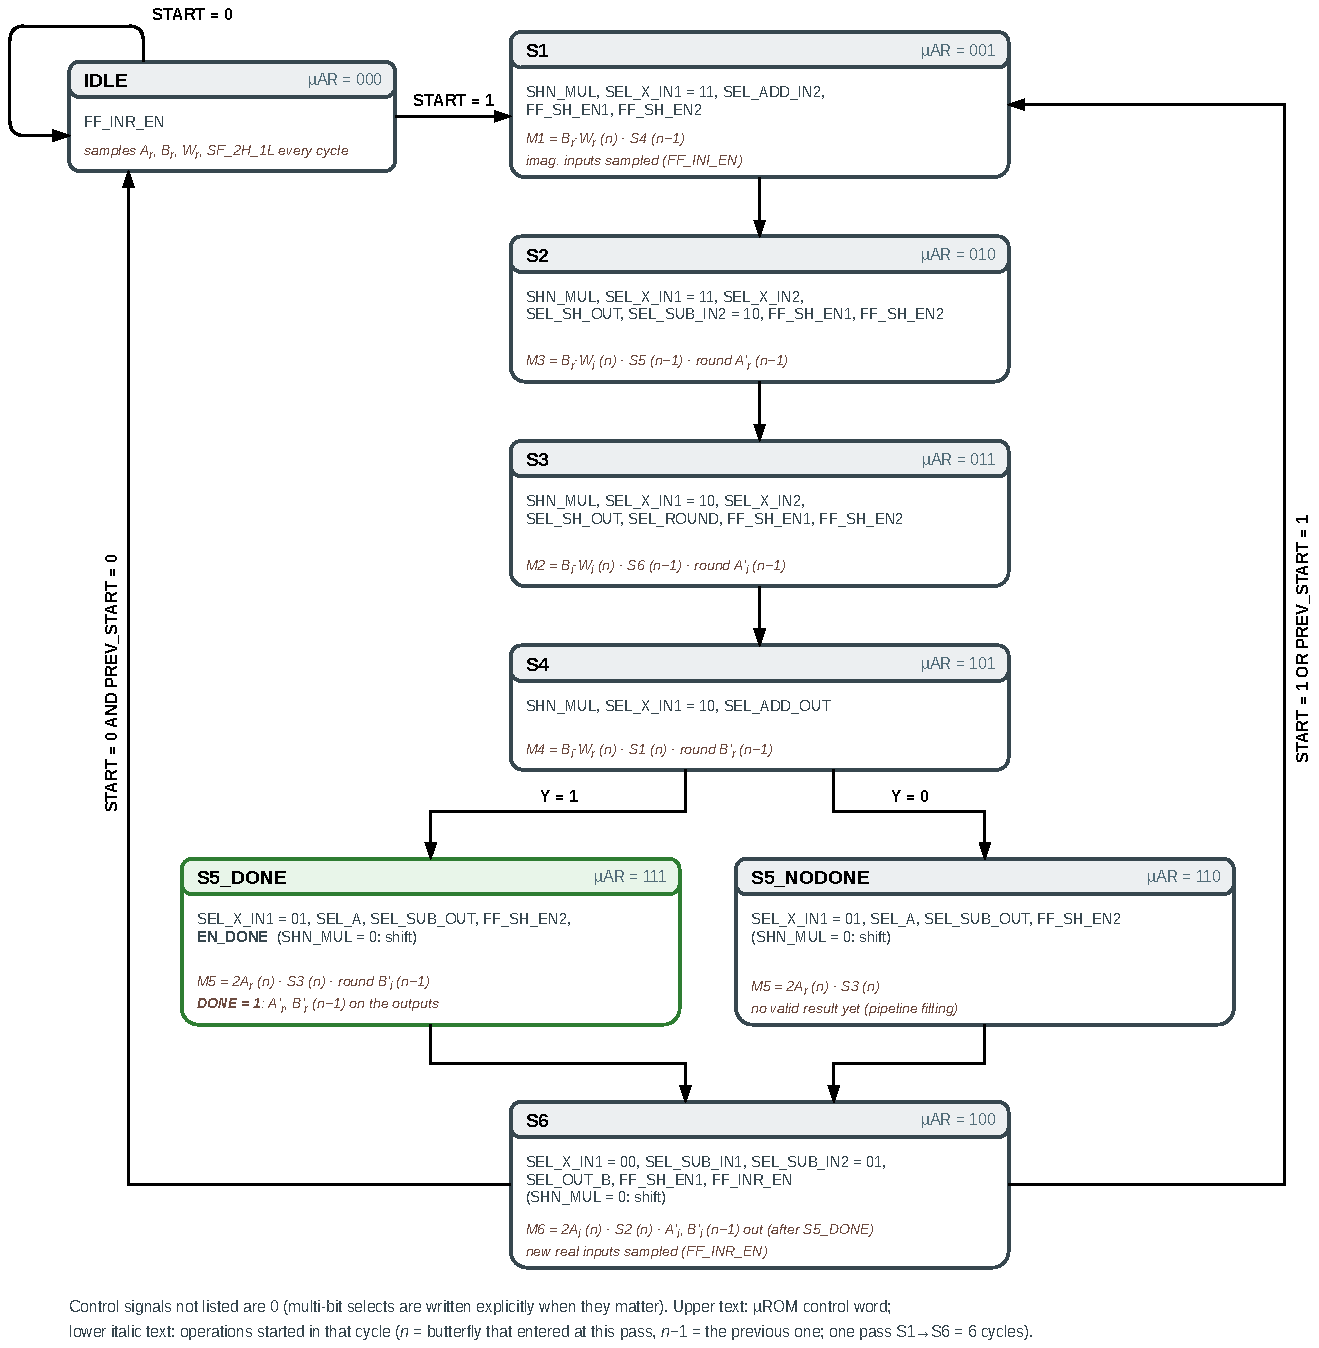
\includegraphics[width=0.93\textwidth]{fig04_state_diagram}
      \caption{Diagramma degli stati della Butterfly}
\end{figure} 
La macchina a stati sviluppata ha lo scopo di coordinare i segnali di controllo del datapath e gestire la sovrapposizione temporale delle operazioni, permettendo anche la modalità continua, come descritto in seguito nella sottosezione \ref{subsec:modalità}. In particolare, per ridurre il numero di stati utilizzati, si è scelto di ottimizzare il flusso di controllo: ciascuno stato gestisce sia l'elaborazione dei nuovi dati in ingresso, sia il completamento delle operazioni relative ai dati acquisiti al precedente segnale di $START$. Infatti, per terminare l'elaborazione degli ingressi, sono necessarie due iterazioni della sequenza di stati che vanno dallo STATO 1 allo STATO 6 (nelle figure indicati in breve come S1, \dots, S6, S5\_DONE e S5\_NODONE), senza che la macchina torni tra le due in IDLE.

\noindent Si specifica che i controlli non indicati per gli stati nello State Diagram riportato sono di default a zero; in questo, si notano 2 segnali non presenti nel datapath, che sono stati introdotti per la gestione dell'evoluzione degli stati della macchina e descritti nella sottosezione \ref{subsec:Y,PREV_START,DONE} : Y e PREV\_START. Di seguito si indica il comportamento della macchina in ciascuno degli stati presentati nel diagramma degli stati (si consiglia di leggere prima la parte relativa al ciclo attuale per ognuno degli stati, e solo alla fine leggere in ordine le descrizioni relative al ciclo precedente, per comprendere al meglio il flusso delle operazioni):
\begin{itemize}
\item Nello stato di IDLE, in cui si permane in attesa che il segnale di $START$ si abiliti, si attiva il segnale FF\_INR\_EN. Anche se la macchina è ferma, si mantiene abilitata la scrittura dei dati di input. In tal modo, si può risparmiare un ciclo di clock, poiché quando START va a uno, in corrispondenza del rising edge del clock avviene la transizione allo STATO 1 e sono già stati salvati i valori delle parti reali di $A$, $B$ e $W$. Inoltre, si campiona anche il segnale SF\_2H\_1L.

\item  Nello STATO 1, Ciclo attuale: FF\_INI\_EN è attivo e perciò le parti immaginarie di $A$, $B$ e $W$ verranno campionate al prossimo fronte di salita. SEL\_X\_IN1 =  11 instrada verso il blocco moltiplicatore $B_{r}$, mentre SEL\_X\_IN2 = 0 permette di selezionare come altro termine del prodotto $W_{r}$. Mandando ad uno il segnale SHN\_MUL, si può eseguire il prodotto $M_1 =B_{r} \cdot W_{r}$. 

\noindent Ciclo precedente: inizia la somma $S_4$ con i dati del precedente ciclo; per tale ragione, SEL\_ADD\_IN2 è impostato alto, così da indirizzare all'ingresso del sommatore $S_3$ l'ingresso voluto. Si attivano pure i segnali di enable dei due registri in cascata in uscita dallo shifter aritmetico, al fine di poter salvare il risultato di $M_6$ al prossimo fronte di salita e traslare nel secondo registro quello di $M_5$, ricavato nella precedente iterazione. Invece, SEL\_SUB\_OUT = 0, per poter salvare nel registro sottostante al sottrattore il risultato di $S_2$.

\item Nello STATO 2, Ciclo attuale:  tramite SEL\_X\_IN1 =  11, si instrada verso il blocco moltiplicatore $B_{r}$, mentre, grazie a SEL\_X\_IN2 =  1,  $W_{i}$ viene mandato all'ingresso del moltiplicatore: poiché  SHN\_MUL = 1, si effettua il prodotto $M_3 =B_{r} \cdot W_{i}$. 

\noindent Ciclo precedente: pongo  SEL\_SUB\_IN1  =  0 e SEL\_SUB\_IN2  =  10, per indirizzare i dati necessari per effettuare l'operazione di sottrazione $S_5$. In aggiunta, SEL\_ROUND = 0, per arrotondare e traslare verso destra il risultato $S_2$ (al fine di ottenere l'uscita su 24 bit $A'_r$), che verrà poi instradato verso il primo registro in uscita allo Shifter aritmetico effettuato dal blocco moltiplicatore, grazie a SEL\_SH\_OUT =  1. Poiché SEL\_ADD\_OUT =  1, il risultato dell'operazione $S_4$ verrà diretto verso il registro posto successivamente al sommatore. FF\_SH\_EN1 e FF\_SH\_EN2 sono attivi. 

 
\item  Durante lo STATO 3, Ciclo attuale:  avviene il prodotto $M_2 = B_{i} \cdot W_{i}$; infatti, viene imposto che SEL\_X\_IN1 = 10, SEL\_X\_IN2 = 1 e SHN\_MUL = 1. 

\noindent Ciclo precedente: SEL\_SH\_OUT = 1 e SEL\_ROUND = 1, al fine di arrotondare e shiftare il risultato $S_4$, per ricavare l'uscita su 24 bit $A'_i$ che viene salvata nel registro attualmente occupato da $A'_r$, il quale si sposta nel registro abilitato da FF\_SH\_EN2. Infatti, i segnali di enable FF\_SH\_EN1 e FF\_SH\_EN2 sono attivi. In questo stato viene iniziata anche l'operazione $S_6$, e termina la sottrazione $S_5$.

\item Nello STATO 4, Ciclo attuale: ci si prepara a campionare $M_3$ e si inizia il prodotto $M_4 = B_{i} \cdot W_{r}$, dato che SEL\_X\_IN1 = 10, SEL\_X\_IN2 = 0 e SHN\_MUL = 1. 
Inoltre, i controlli sono tali da fare iniziare la somma $S_1$.

\noindent Ciclo precedente:  terminano le operazioni $S_6$, si campiona $S_5$ e  poiché SEL\_ROUND = 0 e SEL\_ADD\_OUT = 1, si manda ad arrotondare $S_5$ e si ottiene il risultato su 24 bit $B'_r$, il quale è pronto per essere salvato dal registro presente all'uscita del sommatore.
Si disattivano i registri in cascata allo shifter aritmetico per non perdere i valori in essi salvati di $A'_r$ e $A'_i$.

\noindent Da questo stato è presente un salto a due vie,  dipendente dal valore della  variabile Y. Se Y = 1, i dati il cui trattamento è iniziato nell'iterazione precedente sono pronti per essere trasmessi dal prossimo colpo di clock: si passa allo STATO 5\_DONE. Invece, se Y = 0, i risultati non sono ancora pronti; si transisce, di conseguenza, allo STATO 5\_NODONE.

\item  Nello STATO 5 (sia \_DONE che \_NODONE): si ha il set degli enable per campionare, al prossimo rise, le operazioni $S_1$ e $M_2$;  viene iniziato il calcolo della somma $S_3$, dato che  SEL\_A = 1 e SEL\_ADD\_IN2 = 0. Dal momento che SEL\_X\_IN1 =  01 e SHN\_MUL = 0, si verifica lo shift di $A_{r}$ ($M_5 = 2A_{r}$).

\noindent Ciclo precedente: si manda ad arrotondare $S_6$, per ottenere l'uscita $B'_i$, pronta ad essere salvata nel registro a valle del sottrattore.

\noindent Nello STATO 5\_DONE si attiva il segnale esterno DONE, dato che EN\_DONE = 1 e Y = 1. In questo stato, la butterfly manda verso l'esterno due segnali validi su 24 bit, ovvero le parti reali dei risultati dell'elaborazione. Nello STATO 5\_NODONE, invece, EN\_DONE =  0: non viene generato alcun segnale di DONE, poiché non si hanno dati pronti. 


\item  Nello STATO 6, entrambi i cicli: il sommatore, il moltiplicatore e lo shifter aritmetico trasmettono alla loro uscita, rispettivamente, i risultati delle operazioni $S_3$, $M_4$ e $M_5$; per tale ragione, FF\_SH\_EN1 = 1, SEL\_SH\_OUT = 0 e SEL\_ADD\_OUT = 0. Inoltre, avendo SEL\_X\_IN1  = 00 e SHN\_MUL = 0, viene iniziato il calcolo dello shift aritmetico della parte immaginaria di A ($M_6$). Oltre a ciò, viene avviata la sottrazione $S_2$, poiché SEL\_SUB\_IN1 = 1 e SEL\_SUB\_IN2 = 01.
In tale stato, inoltre, si imposta FF\_INR\_EN = 1: ciò è necessario per campionare i nuovi input $A_r$, $B_r$, $W_r$ e SF\_2H\_1L, nel caso in cui la macchina funzioni in modalità continua. In aggiunta, se lo stato precedente della macchina era STATO 5\_DONE, in uscita vengono inviati i risultati $A'_i$ e $B'_i$ (grazie al fatto che SEL\_OUT\_B = 1).
Se si verifica la condizione (PREV\_START) OR (START), la macchina non finisce in IDLE al successivo colpo di clock, bensì salta direttamente allo STATO 1. Infatti, se uno dei due operandi della OR logica è alto, indica che è necessaria almeno un'altra iterazione della sequenza di stati STATO 1  -  STATO 6. In caso contrario, si ritorna nello stato di attesa. 

\end{itemize}


\subsection{Analisi di ulteriori segnali generati nella CU}
\label{subsec:Y,PREV_START,DONE}
\noindent Si analizzano ora altri segnali di estrema rilevanza che sono generati all'interno della unità di controllo della Butterfly.

\noindent Per prima cosa, si studia il segnale FF\_INI\_EN. Come già espresso nelle precedenti sottosezioni, quando FF\_INR\_EN risulta alto, si attivano i registri in ingresso all'unità, relativi alle parti reali dei dati in input e quelli legati al segnale che regola lo shift finale verso destra SF\_2H\_1L. Poiché, per il protocollo di comunicazione utilizzato per le Butterfly progettate, si vogliono campionare le parti immaginarie degli ingressi con un colpo di clock di ritardo rispetto alle parti reali, si è deciso di generare il segnale FF\_INI\_EN mediante un flip-flop con ingresso FF\_INR\_EN, con il beneficio di ridurre di uno la dimensione di ogni parola della $\mu ROM$ presente nell'unità di controllo del componente.

\begin{figure}[H]
      \centering
      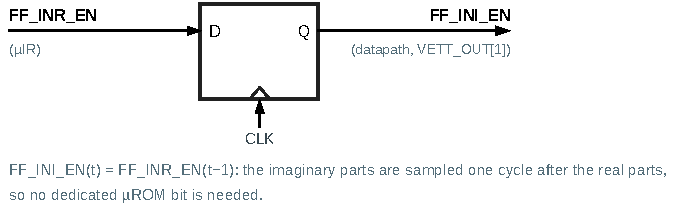
\includegraphics[width=0.7\textwidth]{fig05_ff_ini_en}
      \caption{Logica per la gestione di FF\_INI\_EN}
\end{figure} 

\noindent Invece, per gestire correttamente l'evoluzione dello stato presente della macchina, si è trovato come soluzione l'introduzione di una sorta di segnale di START ritardato. In particolare, si è aggiunto un segnale intermedio START\_INT, che di fatto è esattamente uno START ritardato di un colpo di clock, il quale è utilizzato come ingresso di un registro, che ha come segnale di enable (SEL\_ADD\_IN2) AND (SHN\_MUL). Questa scelta è dovuta al fatto che tale prodotto logico risulta pari a 1 unicamente nello STATO 1. Poiché l'architettura progettata è sensibile unicamente a un segnale di START attivo negli stati IDLE e/o 6, in tale maniera si è implementato un modo per ottenere PREV\_START, che permette di indicare alla macchina, quando si trova in STATO 6, se si era osservato uno START alto nello STATO 6 dell'iterazione precedente della sequenza di stati 1-6; infatti, in tal caso, PREV\_START=1. Nel caso in cui invece si è alla prima iterazione della sequenza di stati, allora certamente il sistema osserverà in STATO 6 che PREV\_START=1.

\begin{figure}[H]
      \centering
      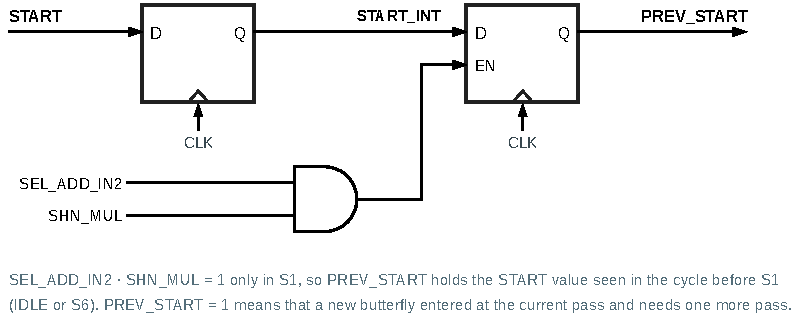
\includegraphics[width=0.85\textwidth]{fig06_prev_start}
      \caption{Descrizione del segnale PREV\_START}
\end{figure} 

\noindent Si introduce, infine, Y, un segnale utile per decidere se, quando la macchina a stati si trova nello STATO 4, deve saltare in STATO 5\_DONE per generare il segnale di fine elaborazione o meno. Se, nel quarto stato, Y risulta pari a 0, la butterfly è in fase di elaborazione, ossia i dati stanno scorrendo nei blocchi operativi del datapath, ma i risultati non sono ancora pronti; di contro, se Y = 1, il processing element è in condizione di fornire in uscita i risultati validi.

\noindent Il segnale Y coincide con l'uscita di un registro Set/Reset. Il Set è stabilito dal segnale SEL\_A, che si attiva unicamente nello STATO 5 (sia in STATO 5\_DONE che 5\_NODONE). 
\noindent La condizione di Reset, al contrario, risulta più complessa: RESET\_Y =  (FF\_INR\_EN AND $\overline{FF\_SH\_EN1}$) OR (START AND $\overline{{PREV\_START}}$ AND FF\_INR\_EN). Il primo termine della somma logica risulta alto in IDLE, così Y è già azzerato quando si attiverà un segnale di START. Inoltre, se arriva un nuovo fronte di salita di START (START = 1 e $PREV\_START$ = 0) mentre FF\_INR\_EN = 1, Y viene azzerato per preparare la nuova computazione. 

\noindent Attraverso l'uso di questo segnale così caratterizzato, si evita che dei dati assolutamente non voluti vengano validati e forniti in uscita erroneamente. 

\noindent Il segnale di DONE si ottiene invece dall'operazione logica di 'AND' tra il segnale EN\_DONE, attivo solo nello STATO 5, e Y. Di conseguenza, il DONE diventa alto solo se le parti reali dei risultati sono pronte a essere forniti in uscita.

\begin{figure}[H]
      \centering
      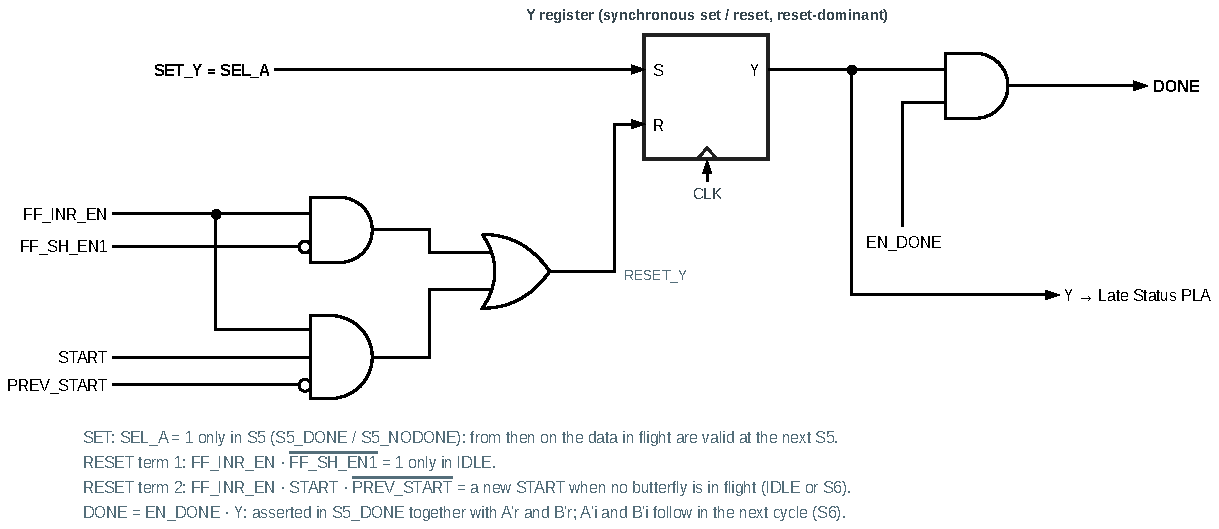
\includegraphics[width=1\textwidth]{fig07_y_done}
      \caption{Gestione  dei segnali Y e DONE}
\end{figure} 


\subsection{Modalità singola e continua}
\label{subsec:modalità}
\begin{comment}
\begin{figure}[H]
      \centering
      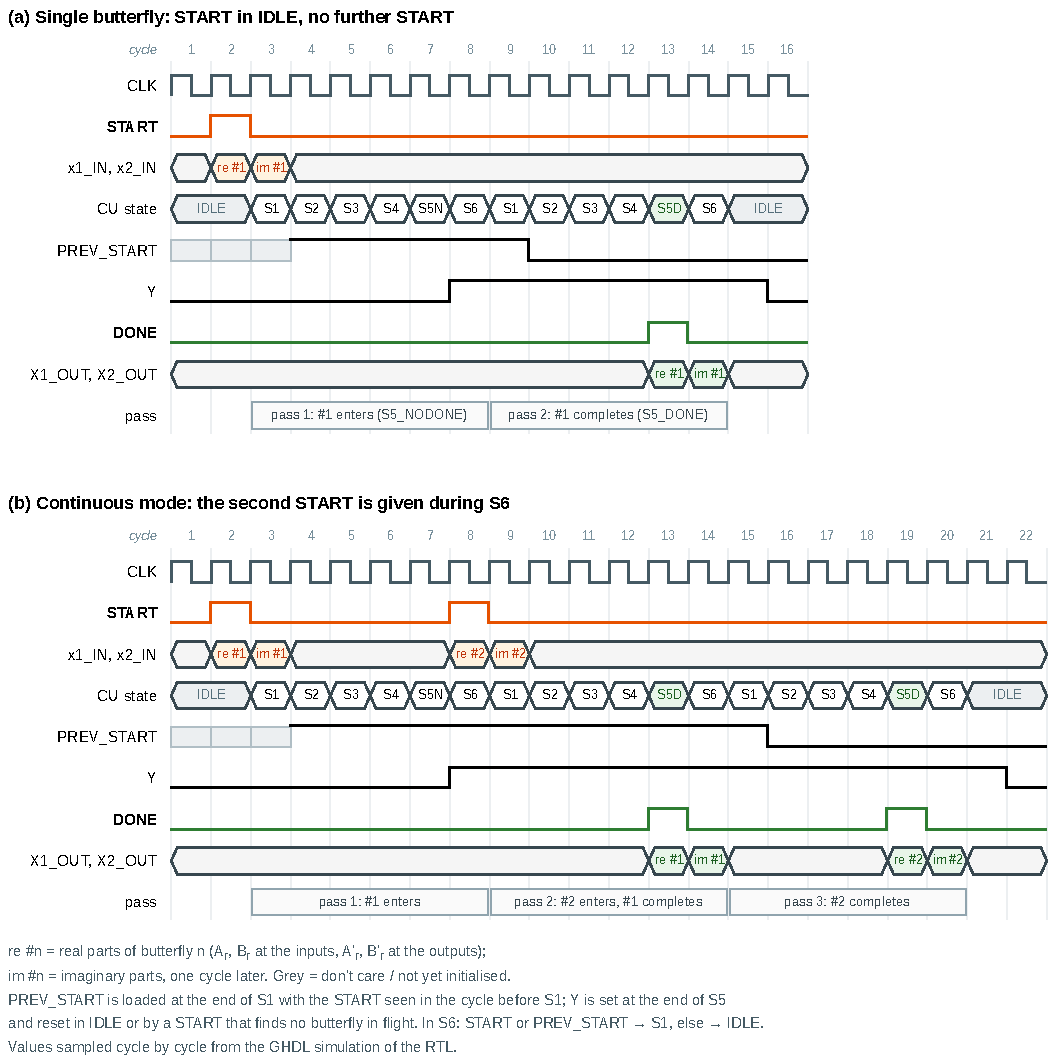
\includegraphics[width=0.7\textwidth]{fig12_single_vs_continuous}
      \caption{Rappresentazione temporale del flusso di esecuzione dei due scenari operativi di modalità continua e modalità single-shot}
\end{figure} 
\end{comment}
\noindent In questa sottosezione, si spiegano le due modalità in cui la singola butterfly (e di conseguenza tutto il sistema che permette di calcolare la FFT su 16 campioni) può lavorare.

\noindent In modalità singola, si elabora un solo pacchetto di dati per volta. Se ad esempio si parte dallo stato di IDLE, nel momento in cui arriva un nuovo START, inizia l'elaborazione dei dati in ingresso, poiché la macchina transita nello STATO 1. Quando lo stato corrente diventa lo STATO 4, si ha che $Y$ è a 0 (poiché azzerato in IDLE) e perciò la macchina passa per lo STATO 5\_NODONE, dato che si devono calcolare i nuovi valori. Dopodiché, la macchina transita in STATO 6 e Y risulta ora forzato a 1 (poiché, in STATO 5\_NODONE, SEL\_A = 1). Nel caso di modalità singola, si ha che il segnale di START in ingresso deve essere basso in questo stato. In questa istanza, si ha che, dallo STATO 6, si transita allo STATO 1, dato che, nonostante lo START disabilitato, PREV\_START vale 1. 
\noindent A questo punto, quando la macchina raggiungerà lo STATO 4, salterà in STATO 5\_DONE, fornendo in uscita le parti reali dei risultati. Al colpo di clock successivo, la macchina si trova in STATO 6 e rende disponibile in uscita le parti immaginarie ottenute dall'elaborazione. Se non si hanno altri segnali di inizio, poiché PREV\_START risulta ora pari a 0, la macchina torna in IDLE, terminando il trattamento.

\vspace{0.5cm}

\noindent La seconda modalità disponibile, quella continua, permette di aumentare il throughput dei dati in uscita. Infatti, l'idea alla base di tale modalità è che, in accordo con il Data Flow Diagram, ogni sei colpi di clock è possibile fornire dei nuovi dati di ingresso alla butterfly e iniziare la nuova elaborazione, in parallelo alla precedente che deve ancora essere completata. Ciò è permesso grazie al fatto che, dopo sei tempi di ciclo del segnale di sincronizzazione, il moltiplicatore è libero di procedere con nuove operazioni, poiché sono già state avviate le 6 moltiplicazioni richieste per l'elaborazione. Inoltre, dopo tale intervallo temporale, non sono più necessari gli ingressi precedenti, per terminare la processazione dei dati antecedenti. 

\noindent Se ad esempio si vuole entrare in modalità continua partendo dallo stato di IDLE, si procede in modo analogo al caso single-shot, con la differenza che, quando la macchina transita per la prima volta in STATO 6, si deve fornire in ingresso un valore alto del segnale di START, contemporaneamente al valore di SF\_2H\_1L e delle parti reali di $A$,$B$ e $W$. Il PE riparte dallo STATO 1, senza ritornare in IDLE, e PREV\_START rimane a 1. Inoltre, il Reset di Y non viene abilitato, permettendo il passaggio per lo STATO 5\_DONE. Attraverso questa procedura, che può essere iterata un numero arbitrario di volte, semplicemente alzando lo START quando la macchina giunge in STATO 6, è quindi possibile ricevere periodicamente dati in ingresso e produrre dei risultati validi ad ogni loop, ovvero ogni sei colpi di clock.

\noindent Quando dall'esterno lo START viene abbassato, la macchina itera ancora una volta la sequenza degli stati e finisce l'elaborazione corrente, poiché è ancora verificato che PREV\_START = 1 al momento della decisione del salto a 2 vie nello stato 6. Dal momento che Y risulta essere ancora 1, in quest'ultima iterazione si transita nuovamente in STATO 5\_DONE; nello stato successivo, poiché PREV\_START = 0, si prende la decisione di tornare nello stato di attesa, nel caso di assenza di attivazione dello START. \\

\noindent Si evidenzia che la soluzione proposta è molto versatile: infatti, grazie alla gestione del salto presente in STATO 6 e dell'implementazione dei segnali Y e PREV\_START descritti in precedenza, è possibile iniziare nuovamente un'elaborazione dati anche dallo STATO 6, senza la necessità di transire in IDLE. In questo modo, è possibile risparmiare un colpo di clock di latenza in alcune condizioni. Ad esempio, si ha la possibilità di avviare un'elaborazione singola, al termine di una processazione in modalità continua, mentre la macchina si trova ancora in STATO 6 e trasmette in uscita gli ultimi risultati $A'_i$ e $B'_i$ della modalità continua, senza necessità di tornare in IDLE. Ciò è garantito dal fatto che, nella situazione descritta, la macchina transita allo STATO 1 e Y viene resettato prima di uscire dallo stato 6, poiché FF\_INR\_EN  = 1, START = 1 e PREV\_START = 0.

\section{Unità di Controllo microprogrammata}

\begin{figure}[H]
      \centering
      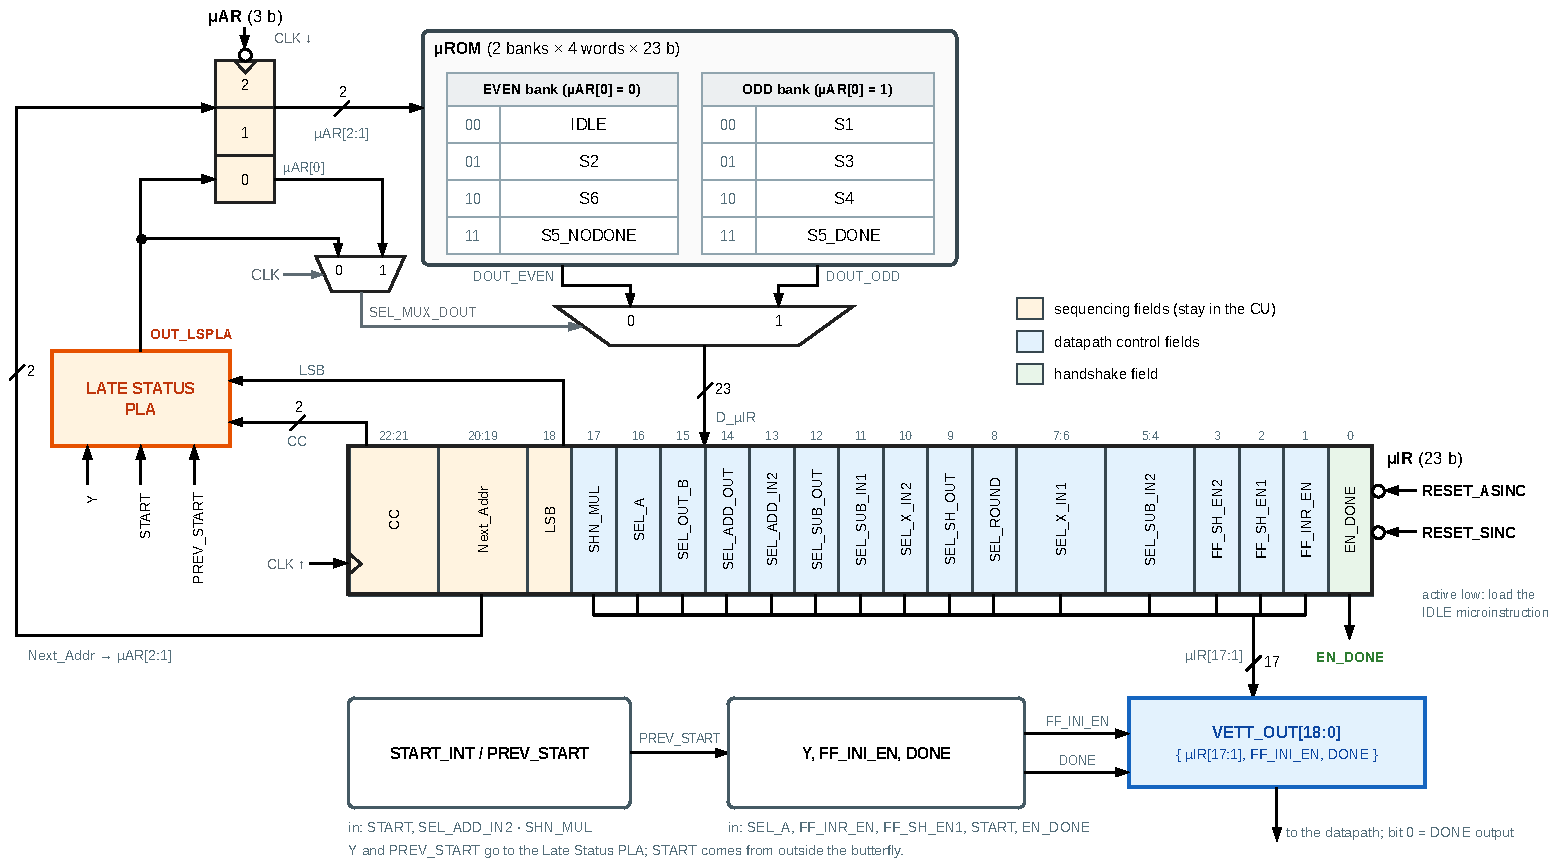
\includegraphics[width=1\textwidth]{fig08_cu_microprogrammed}
      \caption{Schema della CU microprogrammata}
      \label{fig:CU_uProg_schema}
\end{figure} 

\noindent Il diagramma degli stati presentato nella precedente sezione è stato descritto in VHDL attraverso una Unità di Controllo microprogrammata, in cui si è utilizzata la tecnica del LATE STATUS. L'architettura è costituita da quattro elementi fondamentali: la $\mu ROM$, il registro dei micro-indirizzi $\mu AR$, il registro in cui vengono salvate le $\mu$Istruzioni $\mu IR$ ed il blocco logico di selezione.

\noindent Il registro $\mu AR$, il quale si è scelto che campioni sul fronte di discesa del clock, memorizza la codifica dello stato (e quindi il $\mu$indirizzo) corrente. In particolare, il $\mu AR$ ha un parallelismo di 3 bit, poiché la codifica degli stati avviene su soli 3 bit, dato che nello State Diagram sono presenti 8 stati distinti.

\noindent La micromemoria, caratterizzata da un indirizzo su due bit, è divisa in due banchi da 4 locazioni ciascuna: quello delle righe pari, che racchiude le microistruzioni relative agli indirizzi con LSB=0 e quello delle righe dispari (relative agli indirizzi per cui LSB=1). Ogni parola contiene una microistruzione da 23 bit. 

\noindent Invece, il registro $\mu IR$, caratterizzato dal medesimo parallelismo delle parole della $\mu ROM$, campiona sul fronte di salita del segnale di sincronizzazione la $\mu$Istruzione selezionata.

\noindent Infine, la logica di Selezione, formata dalla Late Status PLA e da due multiplexer, decide se verrà eseguita l'istruzione associata all'indirizzo pari o a quello dispari. Infatti, quando il $\mu AR$ punta ad una riga della memoria, vengono lette contemporaneamente entrambe le microistruzioni possibili dai due banchi. La parola voluta viene selezionata da un multiplexer, che ha come selettore l'uscita della PLA, che coincide con il LSB della codifica del prossimo stato. In particolare, tale bit viene anche salvato, in corrispondenza del falling edge del clock, nel bit meno significativo del $\mu$AR. Per questo si è implementato un secondo multiplexer, pilotato dal clock stesso, che sceglie da dove prendere il selettore della prossima $\mu$Istruzione SEL\_MUX\_DOUT. Quando il clock è basso, ossia dopo il fronte di discesa e fino al fronte di salita successivo, il multiplexer secondario instrada direttamente l'uscita della Late Status PLA (OUT\_LSPLA): in questo modo, sul fronte di salita, il $\mu IR$ campiona la $\mu$Istruzione scelta con il valore più aggiornato dei segnali di stato. Invece, quando il clock è alto (dal fronte di salita fino al fronte di discesa successivo), il multiplexer secondario è girato sull'ingresso opposto e instrada il bit meno significativo salvato nel $\mu$AR.

\noindent Al fine di gestire in maniera più pulita la definizione della entity della CU e i port map di tale component, si sono raggruppate tutte le uscite dell'unità di controllo in un unico vettore VETT\_OUT, la cui mappatura con segnali significativi è presentata nella tabella a seguire.

\begin{comment}
\begin{figure}[H]
      \centering
      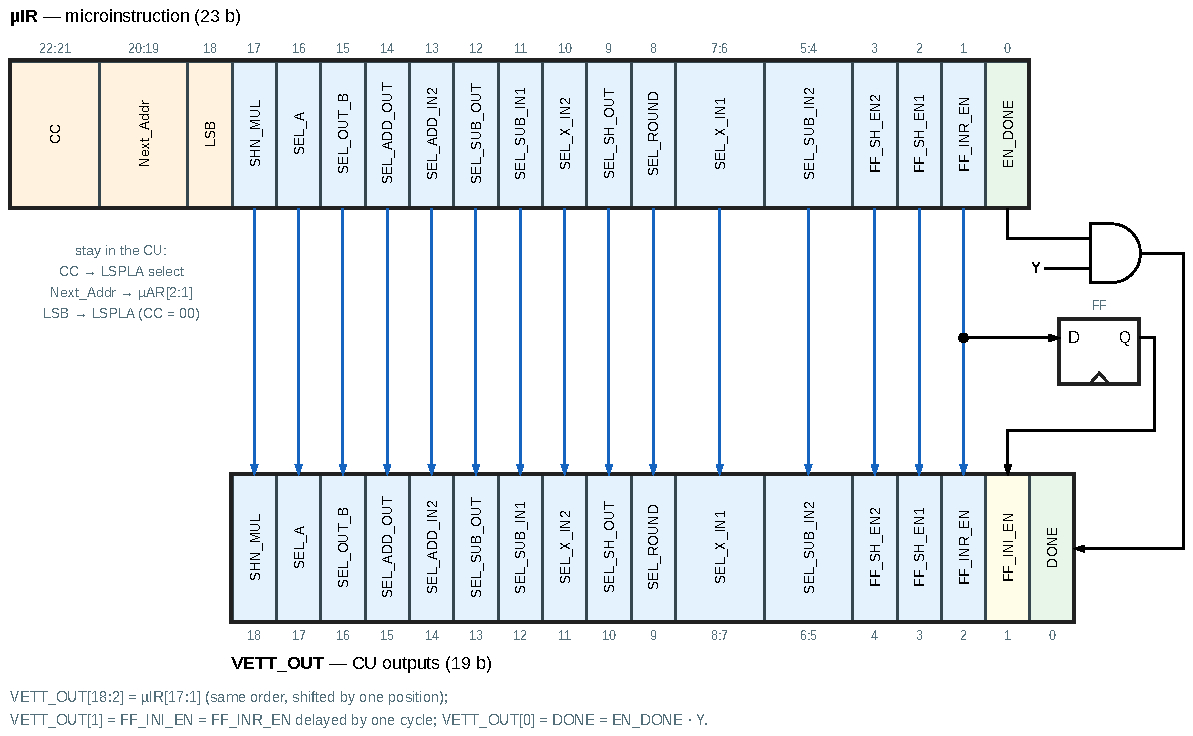
\includegraphics[width=0.9\textwidth]{fig13_microword_vett_out}
      \caption{Tabella che associa, a ciascun bit di VETT\_OUT, il segnale di controllo del datapath }
\end{figure}
\end{comment}

\begin{table}[H]
\centering
\begin{tabular}{|c|l|}
\hline
\textbf{Indice} & \textbf{Nome Segnale} \\ \hline
18 & \texttt{SHN\_MUL} \\ \hline
17 & \texttt{SEL\_A} \\ \hline
16 & \texttt{SEL\_OUT\_B} \\ \hline
15 & \texttt{SEL\_ADD\_OUT} \\ \hline
14 & \texttt{SEL\_ADD\_IN2} \\ \hline
13 & \texttt{SEL\_SUB\_OUT} \\ \hline
12 & \texttt{SEL\_SUB\_IN1} \\ \hline
11 & \texttt{SEL\_X\_IN2} \\ \hline
10 & \texttt{SEL\_SH\_OUT} \\ \hline
9  & \texttt{SEL\_ROUND} \\ \hline
8  & \texttt{SEL\_X\_IN1(1)} \\ \hline
7  & \texttt{SEL\_X\_IN1(0)} \\ \hline
6  & \texttt{SEL\_SUB\_IN2(1)} \\ \hline
5  & \texttt{SEL\_SUB\_IN2(0)} \\ \hline
4  & \texttt{FF\_SH\_EN2} \\ \hline
3  & \texttt{FF\_SH\_EN1} \\ \hline
2  & \texttt{FF\_INR\_EN} \\ \hline
1  & \texttt{FF\_INI\_EN} \\ \hline
0  & \texttt{DONE} \\ \hline
\end{tabular}
\caption{Tabella che associa, a ciascun bit di VETT\_OUT, il segnale di Done o un segnale di controllo da inviare al datapath}
\end{table}

\noindent In conclusione, si evidenzia che il blocco "Y, FF\_INI\_EN, DONE" presente in Figura \ref{fig:CU_uProg_schema}, è composto dalle logiche presentate nella sottosezione \ref{subsec:Y,PREV_START,DONE} per la gestione dei tre segnali indicati.


\subsection{La micromemoria $\mu ROM$}

\begin{comment}
\begin{figure}[H]
      \centering
      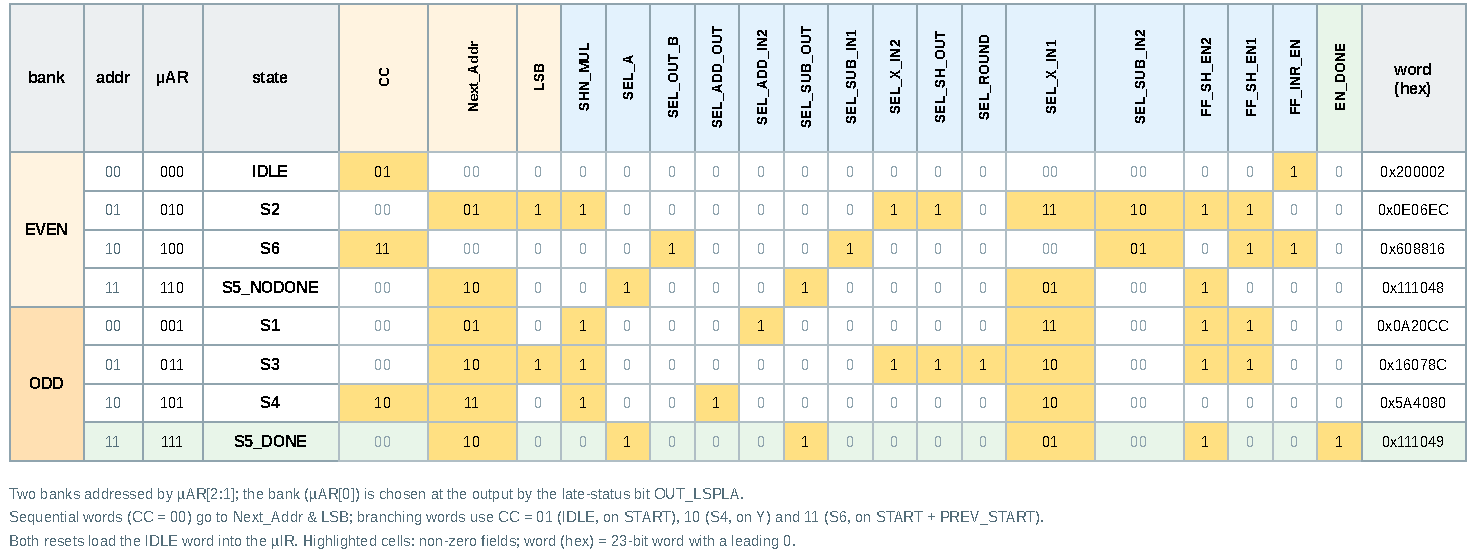
\includegraphics[width=1\textwidth]{fig14_urom_contents}
      \caption{$\mu ROM$}
\end{figure}

\end{comment}
\begin{comment}



\end{comment}

\noindent Come precedentemente detto, la $\mu ROM$ implementata presenta due diversi banchi di memoria: uno per le locazioni pari, e uno per gli indirizzi dispari. Poiché, come evidente dal diagramma degli stati, si hanno in totale $2^3  =  8$ stati, la loro codifica avviene su 3 bit e ciascun banco della micromemoria ha 4 locazioni; l'indirizzo, invece, è su 2 bit e risulta in comune ai due banchi.

\noindent Ogni parola, che codifica una $\mu$Istruzione della macchina, contiene 23 bit; i primi tre campi (CC, Next\_Addr e LSB) gestiscono la logica di sequenziamento, mentre gli altri rappresentano i segnali di controllo. La seguente tabella mostra la codifica di ciascuna $\mu$Istruzione, per ogni stato della macchina. In particolare, escludendo la prima riga in cui è indicata la codifica dello stato in analisi, nelle righe successive sono indicate le codifiche in binario dei vari segnali. Concatenandoli verticalmente, dall'alto verso il basso, è possibile ottenere il contenuto della parola associata allo specifico stato e presente nella $\mu ROM$ (dall' MSB all' LSB).


\begin{table}[H]
\centering


\setlength{\tabcolsep}{4pt} % Spazio orizzontale tra le colonne
\renewcommand{\arraystretch}{1.2} % Spazio verticale tra 
\begin{tabular}{|l|c|c|c|c|c|c|c|c|}
\hline
\textbf{Segnale} & \textbf{IDLE} & \textbf{ST.1} & \textbf{ST.2} & \textbf{ST.3} & \textbf{ST.4} & \textbf{ST.5\_DONE} & \textbf{ST.5\_NODONE} & \textbf{ST.6} \\ \hline
Codifica Stato & 000 & 001 & 010 & 011 & 101 & 111 & 110 & 100 \\ \hline
CC & 01 & 00 & 00 & 00 & 10 & 00 & 00 & 11 \\ \hline
Next\_Addr & 00 & 01 & 01 & 10 & 11 & 10 & 10 & 00 \\ \hline
LSB & 0 & 0 & 1 & 1 & 0 & 0 & 0 & 0 \\ \hline
SHN\_MUL & 0 & 1 & 1 & 1 & 1 & 0 & 0 & 0 \\ \hline
SEL\_A & 0 & 0 & 0 & 0 & 0 & 1 & 1 & 0 \\ \hline
SEL\_OUT\_B & 0 & 0 & 0 & 0 & 0 & 0 & 0 & 1 \\ \hline
SEL\_ADD\_OUT & 0 & 0 & 0 & 0 & 1 & 0 & 0 & 0 \\ \hline
SEL\_ADD\_IN2 & 0 & 1 & 0 & 0 & 0 & 0 & 0 & 0 \\ \hline
SEL\_SUB\_OUT & 0 & 0 & 0 & 0 & 0 & 1 & 1 & 0 \\ \hline
SEL\_SUB\_IN1 & 0 & 0 & 0 & 0 & 0 & 0 & 0 & 1 \\ \hline
SEL\_X\_IN2 & 0 & 0 & 1 & 1 & 0 & 0 & 0 & 0 \\ \hline
SEL\_SH\_OUT & 0 &0  & 1 & 1 & 0 & 0 & 0 &0 \\ \hline
SEL\_ROUND & 0 & 0 & 0 & 1 & 0 & 0 & 0 & 0 \\ \hline
SEL\_X\_IN1 & 00 & 11 & 11 & 10 & 10 & 01 &01 & 00 \\ \hline
SEL\_SUB\_IN2 & 00 & 00 & 10 & 00 & 00 & 00 & 00 & 01 \\ \hline
FF\_SH\_EN2& 0 & 1 & 1 & 1 & 0 & 1 & 1& 0  \\ \hline
FF\_SH\_EN1 & 0 & 1 & 1 & 1 & 0 & 0 & 0 & 1 \\ \hline
FF\_INR\_EN & 1 & 0 & 0 & 0 & 0 & 0 & 0 & 1 \\ \hline
EN\_DONE & 0 & 0 & 0 & 0 & 0 & 1 & 0 & 0 \\ \hline
\end{tabular}%
%} % chiusura resizebox
\caption{Contenuto di ciascuna $\mu$Istruzione e codifica degli stati della macchina}
\end{table}

\noindent In conclusione, il contenuto della $\mu ROM$ è riportato in modo compatto nella tabella sottostante:

\begin{table}[H]
    \centering
    \begin{tabular}{|c|c|c|}
        \hline
        \textbf{Nome dello stato} & \textbf{Indirizzo associato} & \textbf{Contenuto Locazione} \\
        \hline
        IDLE & 000 & 01000000000000000000010 \\
        \hline
        STATO 1 & 001 & 00010100010000011001100 \\
        \hline
        STATO 2 &  010 & 00011100000011011101100 \\
        \hline
        STATO 3 & 011 & 00101100000011110001100 \\
        \hline
        STATO 4 & 101 & 10110100100000010000000 \\
        \hline
        STATO 5\_DONE & 111 & 00100010001000001001001 \\
        \hline
        STATO 5\_NODONE & 110 & 00100010001000001001000 \\
        \hline
        STATO 6 & 100 & 11000001000100000010110 \\
        \hline
    \end{tabular}
    \caption{Contenuto della $\mu ROM$}
    \label{tab:stati_indirizzi}
\end{table}

\subsection{Late Status PLA}
\noindent Tale rete combinatoria gestisce, come già spiegato, la logica dei salti. Come input, presenta ingressi di stato START, $PREV\_START$, $Y$ ed LSB, ovvero il bit meno significativo associato alla codifica dell'istruzione successiva, nel caso in cui non sia necessario saltare. Il campo CC, il 'Condition Code', è codificato su 2 bit, poiché nel pallogramma sono presenti solo 3 diversi salti a 2 vie, ed esso serve alla Late Status PLA per discriminare di quali segnali tenere conto per generare l'uscita $OUT\_LSPLA$. Tale uscita, nell'architettura progettata, è il LSB della codifica dello stato a cui transire, il quale verrà salvato nella locazione 0 del $\mu AR$ in corrispondenza del fronte di discesa del clock del sistema.

\noindent Si è deciso che il campo CC sia pari a 01 quando nel $\mu IR$ è salvata la riga dei comandi associata allo stato di IDLE; in tal caso, in accordo con lo State Diagram e la codifica degli stati scelta, il segnale di START è il responsabile della scelta. Invece, per lo stato 4, CC  = 10 e l'output della PLA coincide con Y, il cui valore andrà a determinare se verrà compiuto il salto in STATO 5\_DONE o in STATO 5\_NODONE. Di contro, nello STATO 6 (CC = 11) intervengono i segnali $START$ e $PREV\_START$ per decidere se tornare in IDLE o meno. Infine, in tutti gli altri stati il condition code vale 00; in tali stati non sono previsti salti e, di conseguenza, il banco della $\mu ROM$ da selezionare dipende unicamente dal campo $LSB$ salvato nel $\mu IR$ ($OUT\_LSPLA \quad = \quad LSB$).

\noindent Si riporta di seguito il semplice multiplexer che descrive lo schematico della PLA progettata.

\begin{figure}[H]
      \centering
      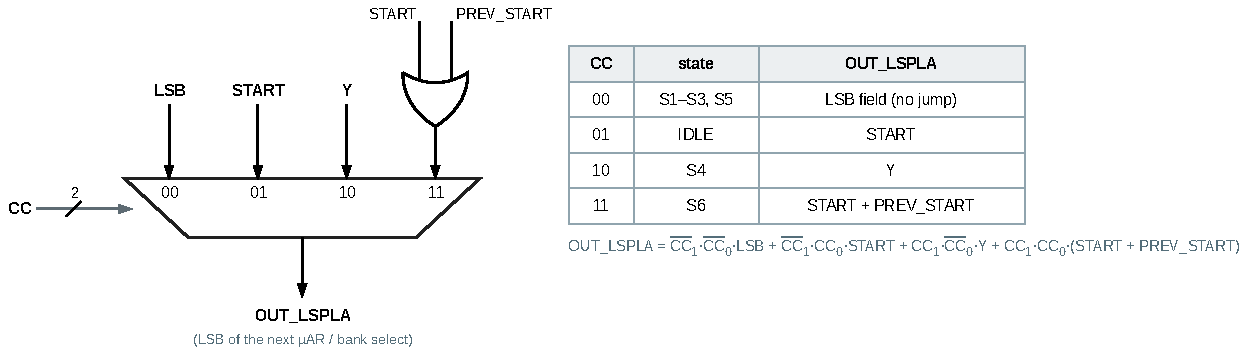
\includegraphics[width=1\textwidth]{fig09_late_status_pla}
      \caption{Schematico del blocco Late Status PLA}
\end{figure}

\noindent Si riportano, per completezza ed a titolo d'esempio, due transizioni logiche del sistema. Per ipotesi, si parte dallo stato di IDLE, con codifica "000". Il campo Next\_Addr vale "00". Dopo che questi due bit vengono salvati nelle prime due locazioni del $\mu AR$, la $\mu ROM$ legge due possibili future righe: quella relativa allo STATO 1 (indirizzo dispari "00(1)") e quella relativa allo IDLE (indirizzo pari "00(0)"). Poiché CC è impostato a "01" in IDLE, la PLA selezionerà il banco pari o dispari a seconda che lo start risulti attivo o meno; la riga scelta verrà salvata nel $\mu IR$ in corrispondenza del fronte di salita seguente del clock.
\noindent Si supponga, invece, che la macchina sia nello STATO 4, per il quale Next\_Addr vale "11". La $\mu ROM$ legge i due possibili percorsi: STATO 5\_DONE (indirizzo dispari "11(1)") o STATO 5\_NODONE (indirizzo pari "11(0)"). La PLA valuta la condizione Y e forzerà OUT\_LSPLA per la selezione dello stato futuro a '0' od a '1'.


\subsection{Reset della Butterfly}
\label{subsec:reset}
La macchina di controllo progettata per la Butterfly, come visibile nella parte destra della Figura \ref{fig:CU_uProg_schema}, presenta due tipologie di reset attivi bassi: uno sincrono e uno asincrono. Quando uno di questi si attiva (quello sincrono deve essere attivo attorno al rising edge del clock), la macchina viene riportata nello stato di IDLE, poiché l'uscita del $\mu IR$ viene impostata pari alla parola della $\mu ROM$ associata allo stato di attesa ("01000000000000000000010").

\noindent In particolare, il reset asincrono è stato introdotto al fine di poter resettare la macchina al power-on, fase in cui il clock potrebbe essere instabile. Questo segnale deve essere utilizzato solo in tale istanza. Invece, il reset sincrono è da utilizzare quando il clock del sistema risulta stabile. Si specifica che, in entrambi i casi, se la macchina viene interrotta mediante uno di questi 2 segnali prima che vengano prodotti i risultati di un'elaborazione, non si osserveranno i corretti dati in uscita negli intervalli temporali in cui sono attesi.

\noindent In conclusione, si indica che la scelta di impostare un valore nel $\mu IR$ rispetto all'azzeramento del $\mu AR$ è dovuta al fatto che, in tale modo, si riesce a essere più reattivi a un futuro segnale di start; infatti, dopo un breve ritardo, la Late Status PLA riceve già i vari bit di controllo associati allo stato di IDLE, al fine di poter generare correttamente il LSB dello stato futuro. Di contro, applicando i reset sul $\mu AR$, sarebbe necessario attendere il fronte di salita successivo al momento in cui il registro viene azzerato, per fornire alla PLA il Condition Code relativo all'IDLE.

\section{Implementazione della FFT e la sua simulazione}

\noindent Una volta verificato il funzionamento dell'unità butterfly, si è implementata la struttura per la FFT, come nell'immagine sottostante.
\noindent \begin{figure}[H]
      \centering
      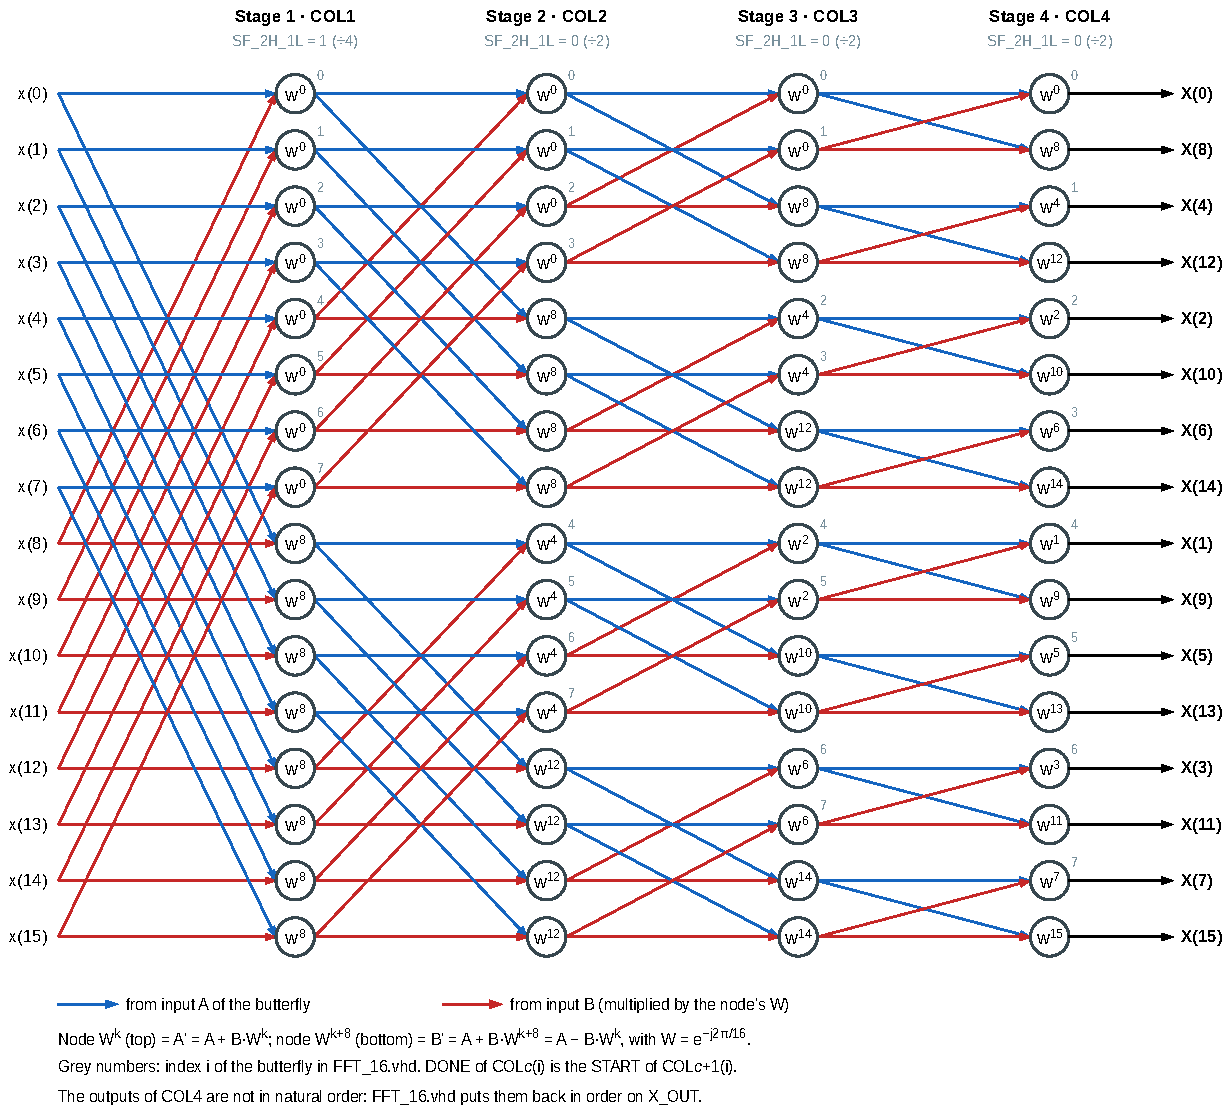
\includegraphics[width=1\textwidth]{fig10_fft16}
      \caption{Schema FFT realizzato}
\end{figure}

\noindent Lo schema evidenzia quattro colonne da 8 butterfly ciascuna, ossia quattro stadi di calcolo, per un totale di 32 butterfly necessarie per compiere una FFT.

\noindent Nel primo stadio, si connettono nodi separati di una quantità pari ad otto, ossia si collegano x(0) e x(8), x(1) e x(9) e così via. Si imposta, inoltre, come da specifica, che solo in tale stadio SF\_2H\_1L sia alto, per gestire l'overflow iniziale di due bit. Negli stadi successivi, invece, è richiesto che SF\_2H\_1L  sia basso. Poiché il numero totale di shift verso destra effettuati sui dati elaborati è pari a 5 (due al primo stadio, uno in tutti gli altri), ci si aspetta uno scale factor di $2^5 = 32$ sui dati di uscita, ovvero che le uscite ottenute dovranno essere implicitamente moltiplicate per tale quantità, al fine di ottenere i risultati correttamente scalati.

\noindent Superato il primo stadio, il sistema organizza i dati separando i percorsi degli stessi in due sottoinsiemi: le uscite A vengono accoppiate tra loro ed elaborate assieme nelle butterfly della colonna successiva, così come le B. In questo modo, si riesce a dividere il problema originale in due blocchi più piccoli e indipendenti, permettendo agli stadi seguenti di lavorare su sotto-insiemi di dati intermedi più piccoli. Di conseguenza, il numero di sottoinsiemi raddoppia dopo ogni stadio.
In aggiunta, escludendo il primo stadio, i coefficienti W variano tra le varie unità butterfly di una singola colonna. L'ultimo stadio, che collega nodi adiacenti, presenta la massima variabilità dei valori W, dato che ad ogni butterfly è associato un coefficiente di rotazione differente.

\noindent Il file VHDL "FFT\_16" che descrive questa architettura e i collegamenti tra le unità è disponibile nella cartella \texttt{rtl/} della repository. A ciascuna butterfly è stato fornito lo stesso reset asincrono e lo stesso reset sincrono, i quali arrivano dall'esterno; inoltre, è stato inchiodato per ciascuna di esse il segnale SF\_2H\_1L. Al fine di presentare un file più rifinito, si sono definiti dei segnali WR e WI al fine di poter raggruppare i portmap delle unità.
\noindent La testbench della FFT (TB\_FFT\_16, nella cartella \texttt{tb/} della repository) è divisa in due parti. Nella prima si applicano i 6 vettori di test forniti dal docente, i cui risultati sono riportati di seguito; nella seconda si eseguono alcuni test aggiuntivi, ad esempio con ingressi complessi e con l'attivazione del reset sincrono durante un'elaborazione, al fine di verificare il corretto funzionamento dell'architettura anche in questi casi.

\noindent Si procede ora a testare la trasformata di Fourier tramite i 6 vettori di test forniti dal docente, i quali risultano sufficienti a verificarne il comportamento, grazie alla variabilità degli stessi. I dati ottenuti dalle simulazioni risultano compatibili con quanto previsto teoricamente. Di seguito, si allegano i vettori utilizzati per la simulazione della FFT, tenendo conto che, ai fini del testing, si sono considerate unicamente le prime 9 componenti dell'uscita. Nella tabella successiva, si presentano i vettori di test utilizzati, sottolineando che le componenti sono indicate dalla posizione 0 alla 15 in ordine crescente.

\begin{table}[H]
    \centering
    \begin{tabular}{|c|l|}
        \hline
        \textbf{Numero Identificativo} & \textbf{Vettore di Test [0 - 15]} \\
        \hline
        1 & [-1,-1,-1,-1,-1,-1,-1,-1,-1,-1,-1,-1,-1,-1,-1,-1] \\
        \hline
        2 & [-1,0,1,0,-1,0,1,0,-1,0,1,0,-1,0,1,0] \\
        \hline
        3 & [1,0,0,0,0,0,0,0,0,0,0,0,0,0,0,0] \\
        \hline
        4 & [-1,-1,+1,+1,-1,-1,+1,+1,-1,-1,+1,+1,-1,-1,+1,+1] \\
        \hline
        5 & [0.5,0.5,0.5,0.5,0.5,0.5,0.5,0.5,0.5,-0.5,-0.5,-0.5,-0.5,-0.5,-0.5,-0.5] \\
        \hline
        6 & [0,0,0,0,0,0,0,0,0.75,0,0,0,0,0,0,0] \\
        \hline
    \end{tabular}
        \caption{Vettori di test utilizzati per la simulazione}
    \label{tab:vettori_test}
\end{table}

\begin{comment}
\begin{itemize}
    \item \textbf{Test 1: DC Costante (Segnale Continuo)}
    \begin{itemize}
        \item \textbf{Ingresso:} Tutti i 16 campioni fissati a $x[n] = -1.0$ (\texttt{1000...0}).
        \item \textbf{Analisi:} Segnale puramente stazionario; l'energia si concentra nel bin a frequenza zero.
        \item \textbf{Uscita attesa:} 
        \begin{itemize}
            \item Bin $k=0$: Parte reale negativo pari a $-16$ (in formato Q1.23).
            \item Bin $k=1 \dots 15$: Parte reale nulla.
            \item Per tutti i bit: parte immaginaria nulla.
        \end{itemize}
    \end{itemize}

    \item \textbf{Test 2: Onda Sinusoidale Pura} 
    \begin{itemize}
        \item \textbf{Ingresso:} Sequenza periodica $\{0, 1, 0, -1\}$ con periodo pari a $T=4$ campioni.
        \item \textbf{Analisi:} Corrisponde a una sinusoide digitale con frequenza $f = f_s/4$.
        \item \textbf{Uscita attesa:}
        \begin{itemize}
            \item Bit $k=4$ e $k=12$: Picchi di ampiezza puramente immaginaria (frequenza positiva e negativa).
            \item Altri Bit: Valori nulli.
        \end{itemize}
    \end{itemize}

    \item \textbf{Test 3: Impulso Delta Finale} 
    \begin{itemize}
        \item \textbf{Ingresso:} $\delta[n-15]$ (tutti 0 tranne l'ultimo campione pari a $\approx 1.0$).
        \item \textbf{Analisi:} La trasformata di un impulso ritardato ha modulo costante e fase linearmente decrescente.
        \item \textbf{Uscita attesa:}
        \begin{itemize}
            \item Parte reale: Costante per ogni $k$ (valore reale circa $1/32 \approx 0.031$).
            \item Fase: I valori complessi ruotano nel piano di Gauss seguendo l'esponenziale $e^{-j\frac{2\pi}{16}15k}$.
        \end{itemize}
    \end{itemize}

    \item \textbf{Test 4: Onda Quadra (Periodo 4)} 
    \begin{itemize}
        \item \textbf{Ingresso:} Sequenza $\{+1, +1, -1, -1\}$ ripetuta.
        \item \textbf{Analisi:} Simile al test 2, ma con forma d'onda quadra. La componente fondamentale è a $k=4$.
        \item \textbf{Uscita attesa:}
        \begin{itemize}
            \item Bin $k=4, 12$: Picchi principali nella parte reale/complessa a seconda della fase iniziale.
            \item Armoniche superiori: Generalmente nulle o ripiegate (aliasing) a causa della bassa frequenza di campionamento rispetto al segnale.
        \end{itemize}
    \end{itemize}

    \item \textbf{Test 5: Onda Rettangolare Lunga} 
    \begin{itemize}
        \item \textbf{Ingresso:} Segnale asimmetrico (9 campioni a $+0.5$ e 7 campioni a $-0.5$).
        \item \textbf{Analisi:} Il segnale ha una componente DC non nulla e una fondamentale a $k=1$.
        \item \textbf{Uscita attesa:}
        \begin{itemize}
            \item Bin $k=0$: Piccola componente reale positiva (valore netto $1.0/32$).
            \item Bin $k=1, 15$: Picchi principali (fondamentale).
            \item Bin dispari ($3, 5, \dots$): Armoniche decrescenti tipiche dell'onda quadra.
        \end{itemize}
    \end{itemize}

    \item \textbf{Test 6: Impulso Delta Centrale} 
    \begin{itemize}
        \item \textbf{Ingresso:} $\delta[n-8]$ (impulso pari a $0.75$ esattamente a metà finestra).
        \item \textbf{Analisi:} Lo spostamento di $N/2$ nel tempo produce una fase alternata $(-1)^k$.
        \item \textbf{Uscita attesa:}
        \begin{itemize}
            \item Parte Reale: Valori che alternano segno tra bin pari e bin dispari.
            \item Parte Immaginaria: Nulla (poiché l'impulso è sull'asse di simmetria reale).
            \item Ampiezza: Modulo costante pari a $0.75 \times 0.5 = 0.375$ (scalato).
        \end{itemize}
    \end{itemize}
\end{itemize}
\end{comment}

\begin{figure}[H]
      \centering
      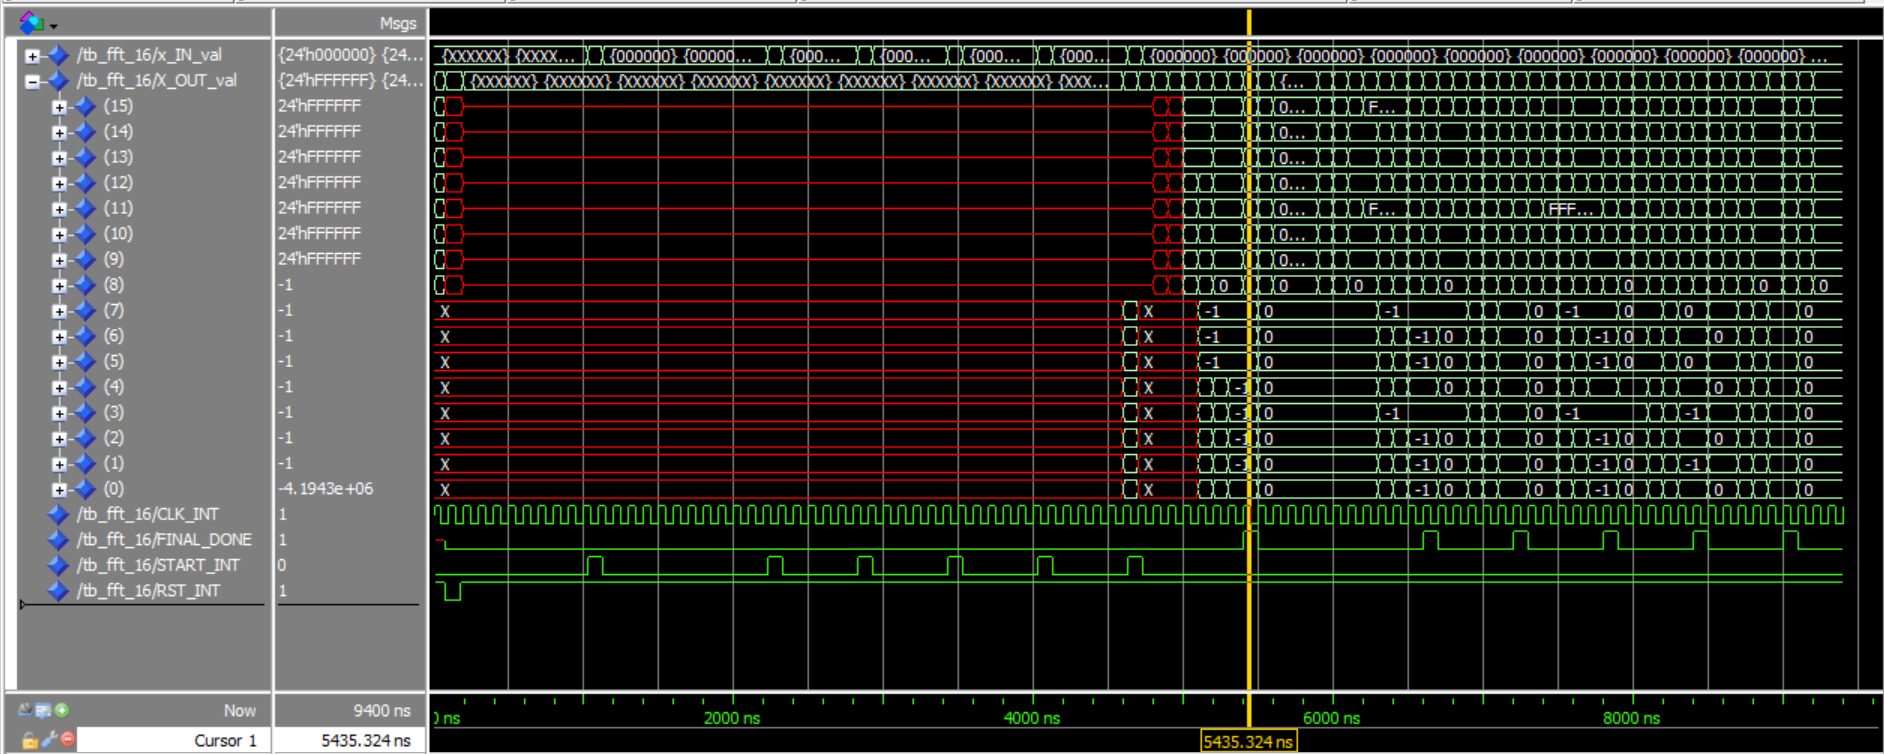
\includegraphics[width=1\textwidth]{sim_tb_fft_16}
      \caption{Schermata della simulazione completa, con focus sulle parti reali dei risultati del test 1}
\end{figure}
\begin{figure}[H]
      \centering
      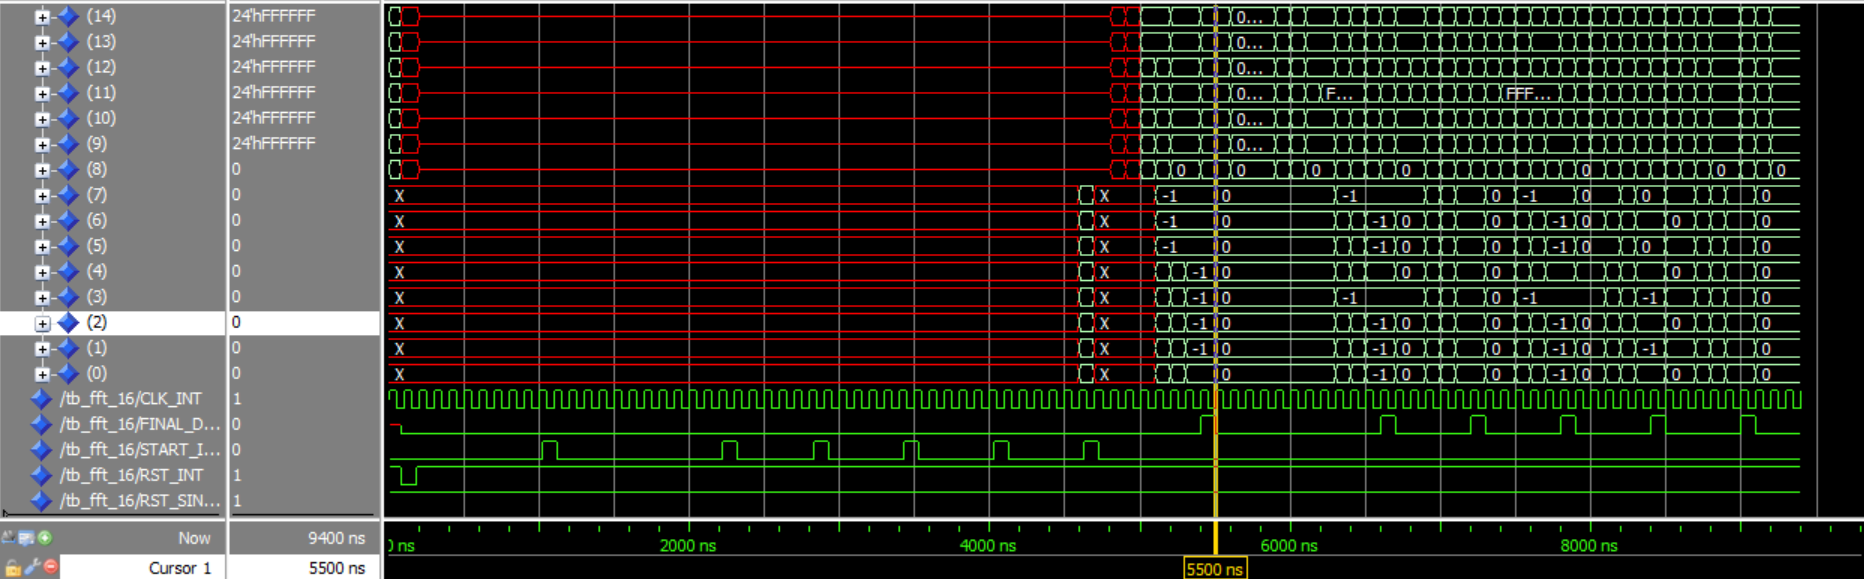
\includegraphics[width=1\textwidth]{sim_test1_imag}
      \caption{Schermata della simulazione completa, con focus sulle parti immaginarie dei risultati del test 1}
\end{figure}
\begin{figure}[H]
      \centering
      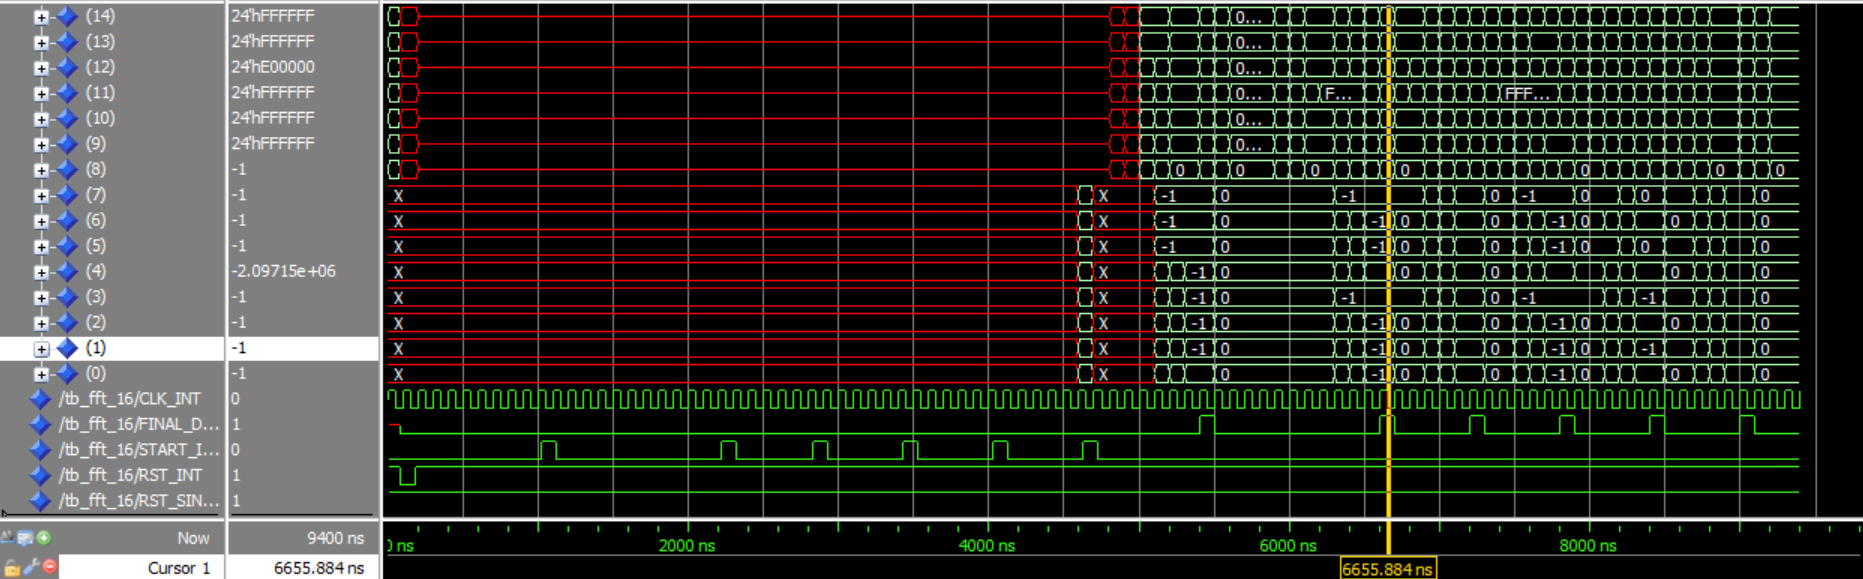
\includegraphics[width=1\textwidth]{sim_test2_real}
      \caption{Schermata della simulazione completa, con focus sulle parti reali dei risultati del test 2}
\end{figure}
\begin{figure}[H]
      \centering
      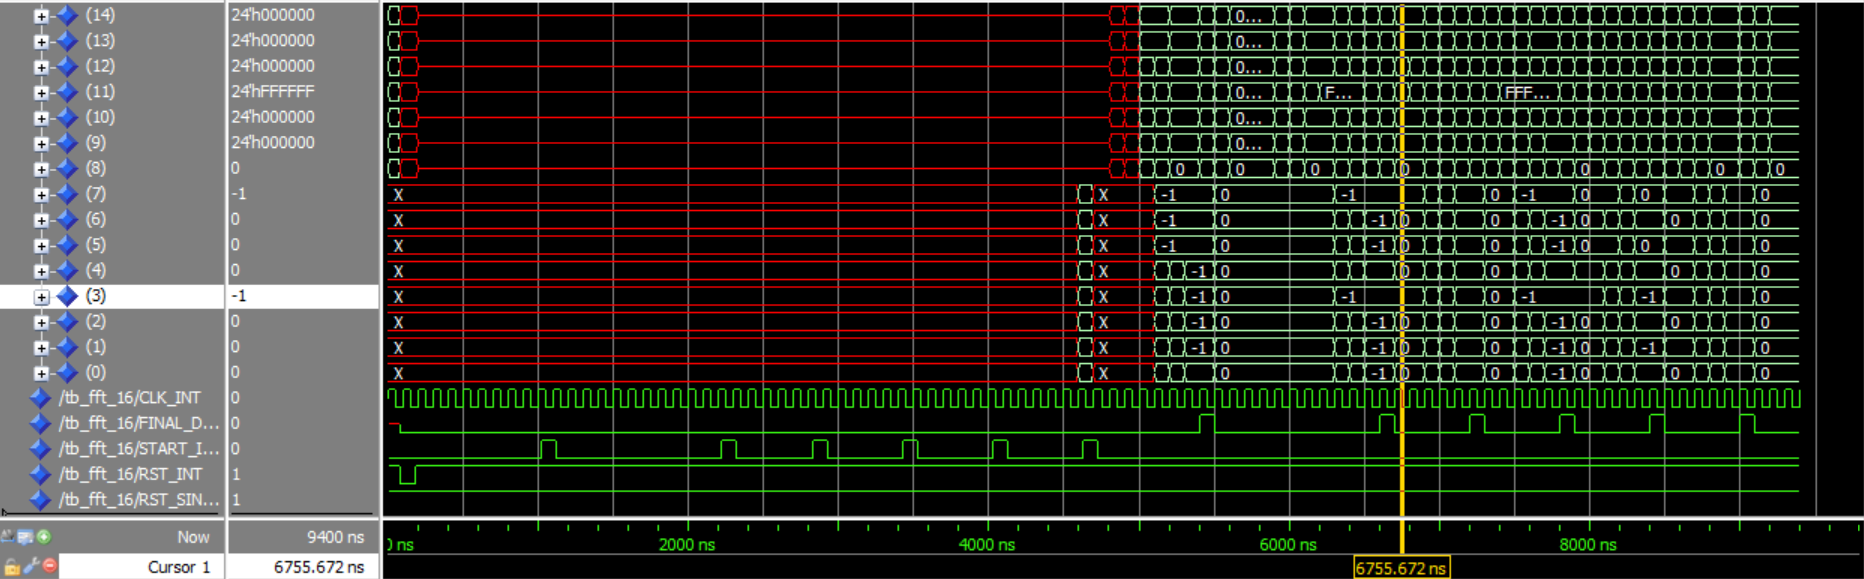
\includegraphics[width=1\textwidth]{sim_test2_imag}
      \caption{Schermata della simulazione completa, con focus sulle parti immaginarie dei risultati del test 2}
\end{figure}
\begin{figure}[H]
      \centering
      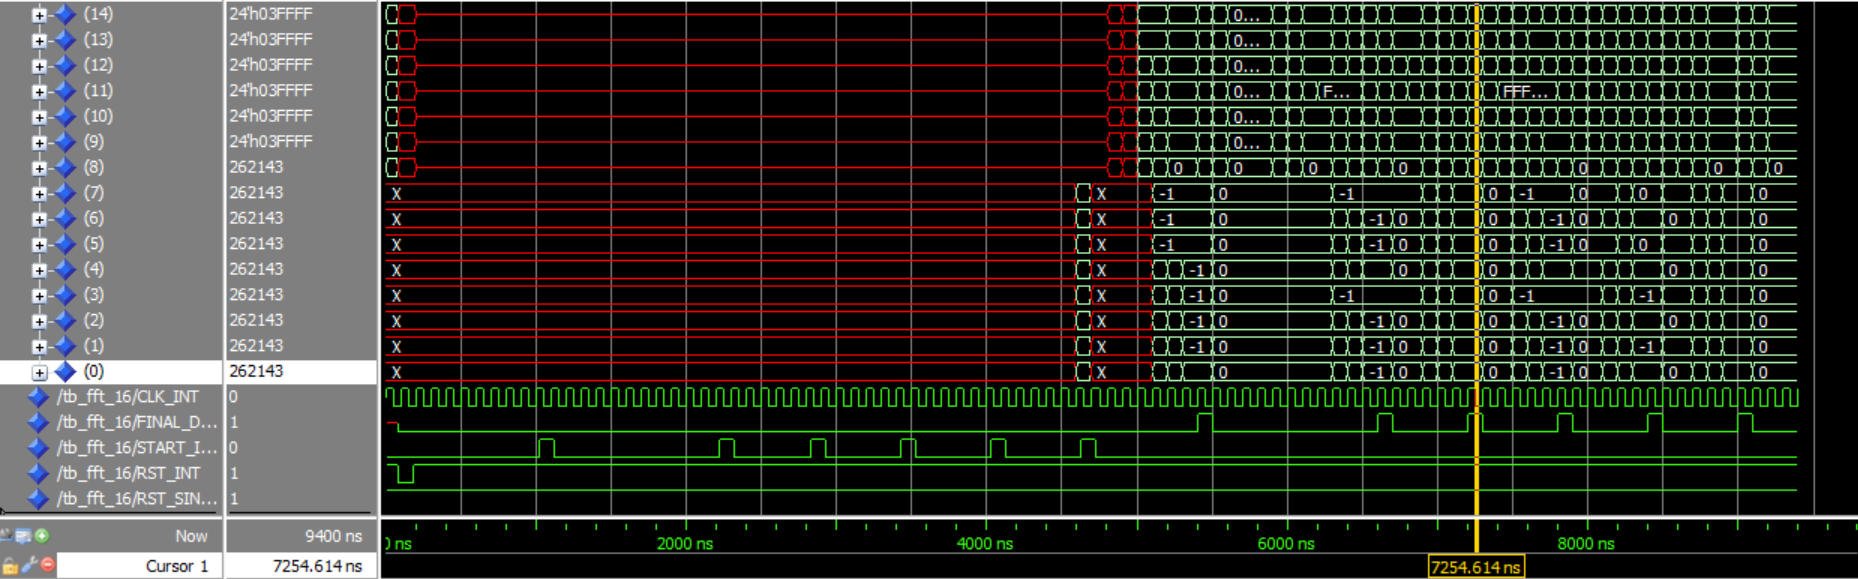
\includegraphics[width=1\textwidth]{sim_test3_real}
      \caption{Schermata della simulazione completa, con focus sulle parti reali dei risultati del test 3}
\end{figure}
\begin{figure}[H]
      \centering
      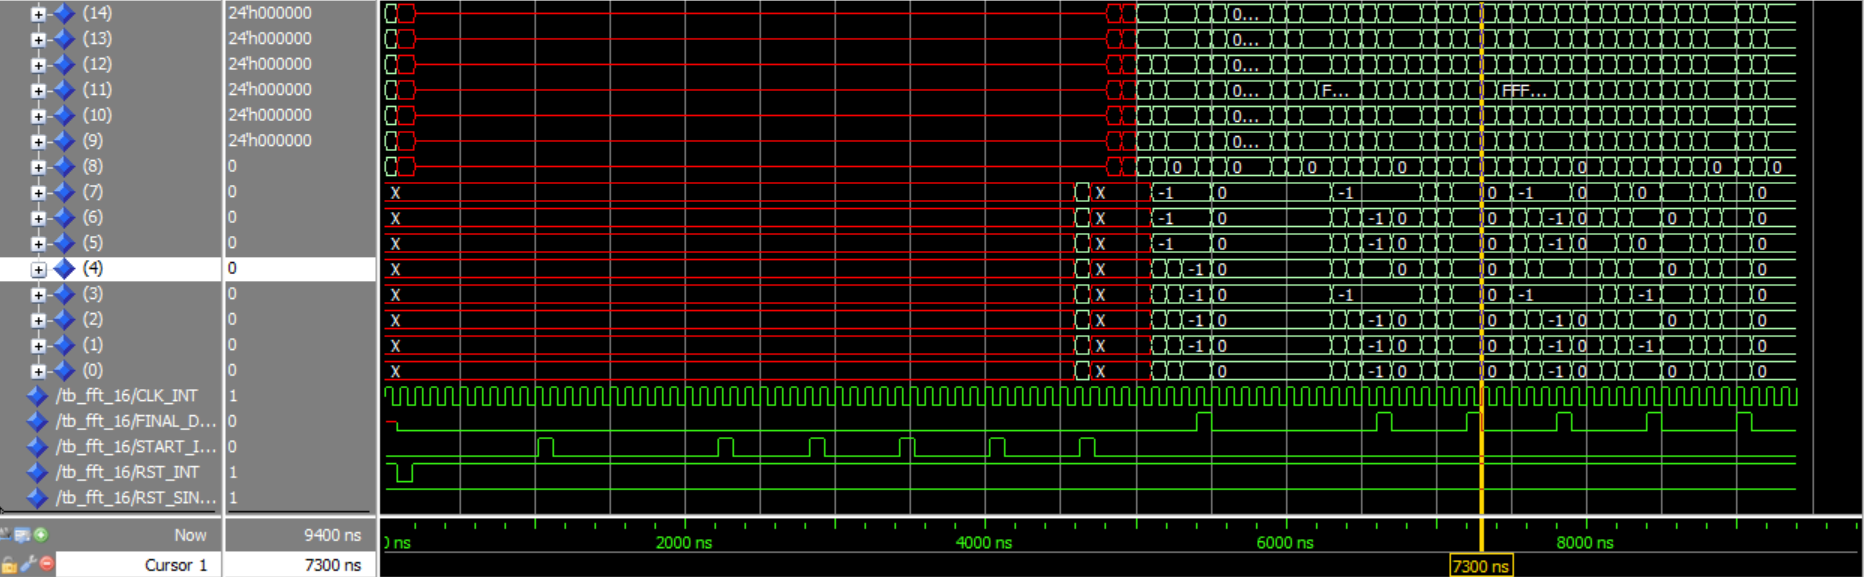
\includegraphics[width=1\textwidth]{sim_test3_imag}
      \caption{Schermata della simulazione completa, con focus sulle parti immaginarie dei risultati del test 3}
\end{figure}
\begin{figure}[H]
      \centering
      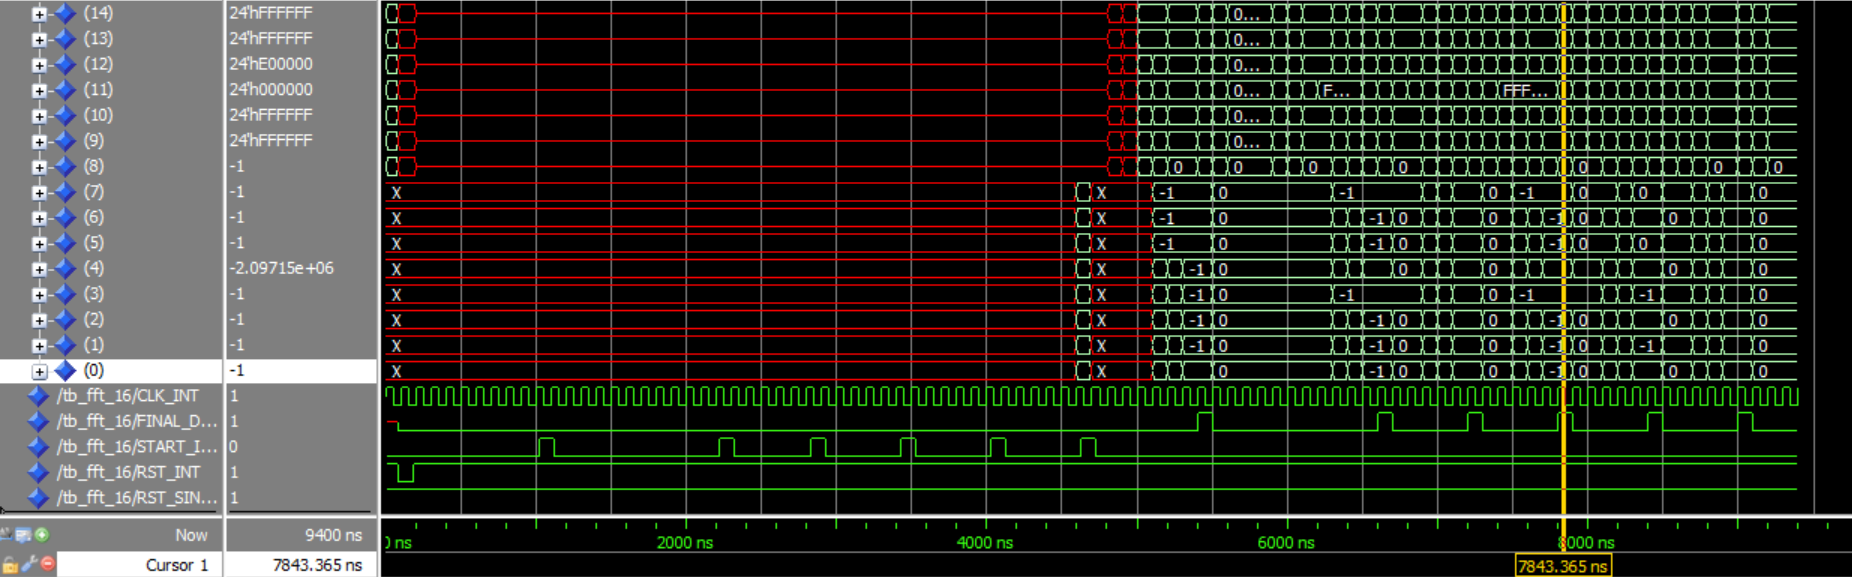
\includegraphics[width=1\textwidth]{sim_test4_real}
      \caption{Schermata della simulazione completa, con focus sulle parti reali dei risultati del test 4}
\end{figure}
\begin{figure}[H]
      \centering
      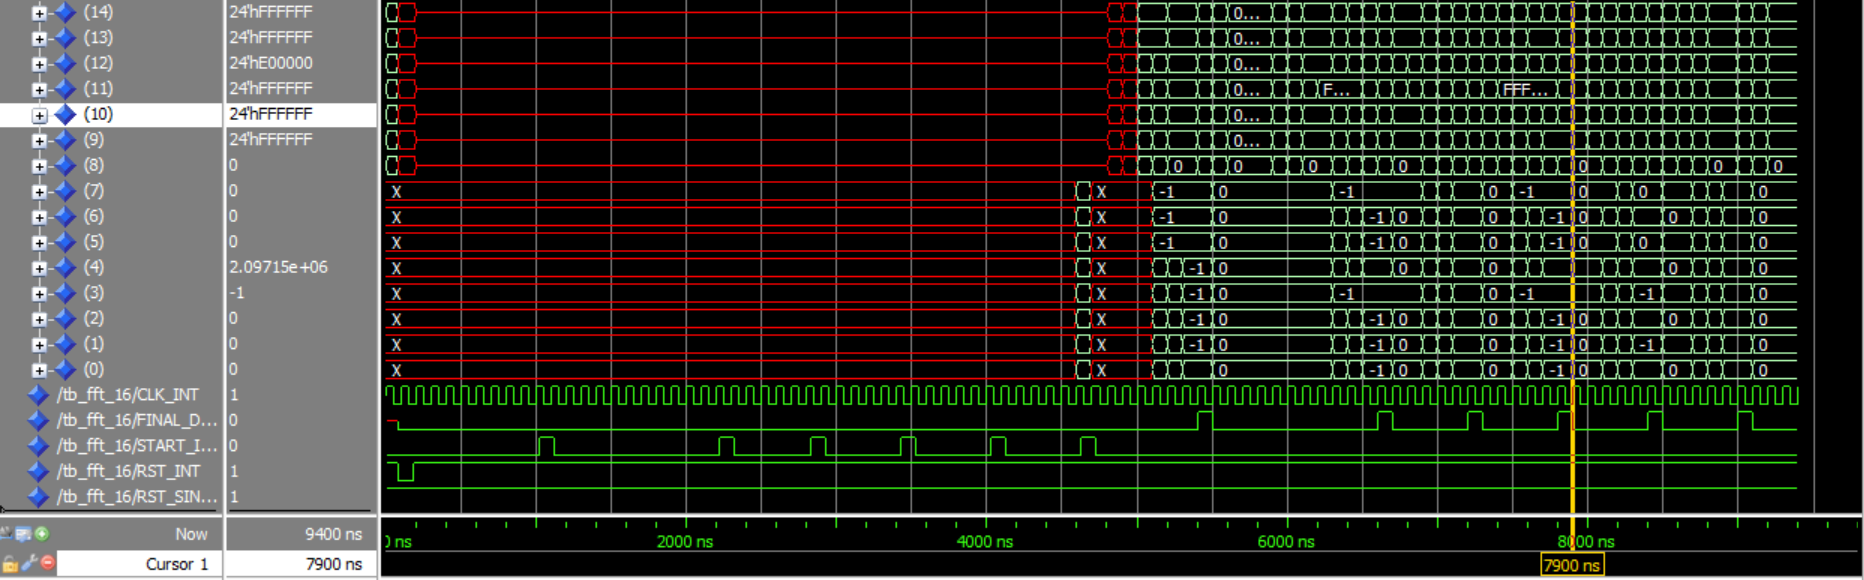
\includegraphics[width=1\textwidth]{sim_test4_imag}
      \caption{Schermata della simulazione completa, con focus sulle parti immaginarie dei risultati del test 4}
\end{figure}
\begin{figure}[H]
      \centering
      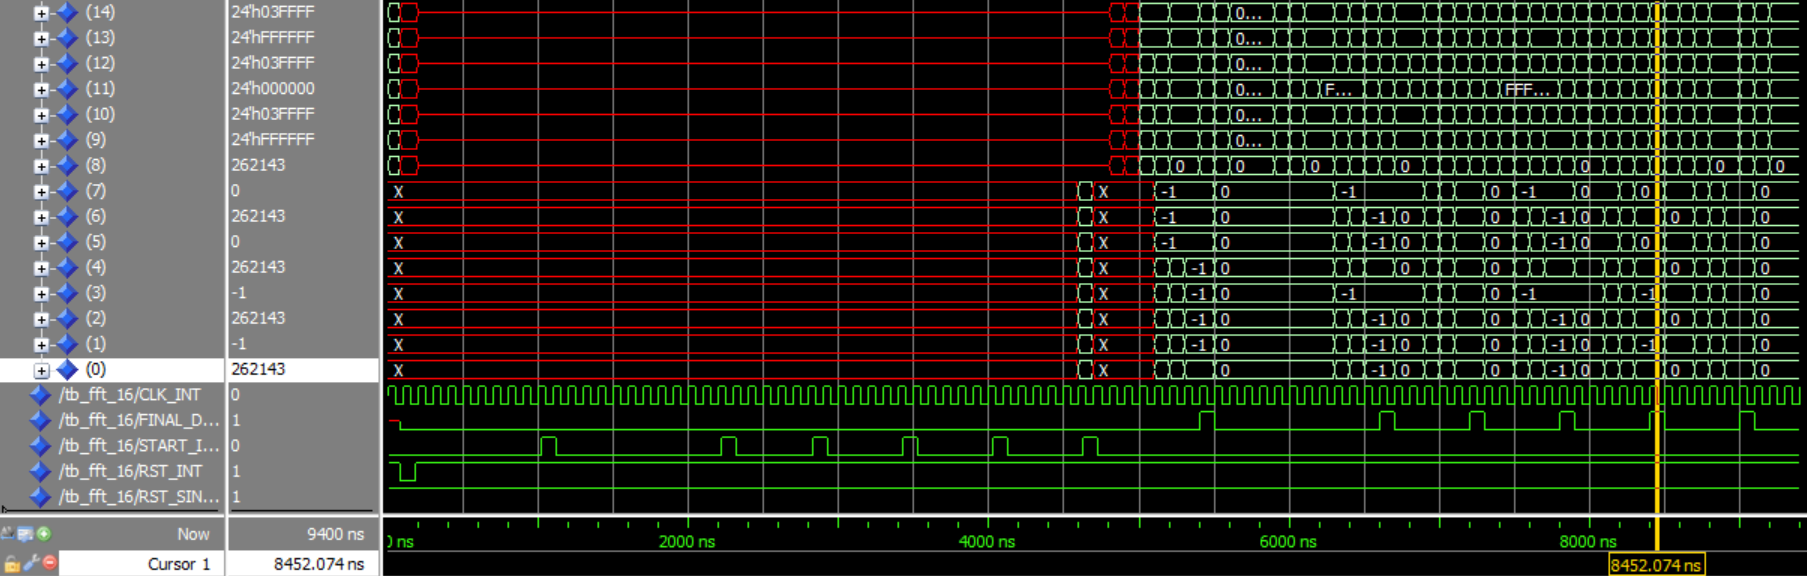
\includegraphics[width=1\textwidth]{sim_test5_real}
      \caption{Schermata della simulazione completa, con focus sulle parti reali dei risultati del test 5}
\end{figure}
\begin{figure}[H]
      \centering
      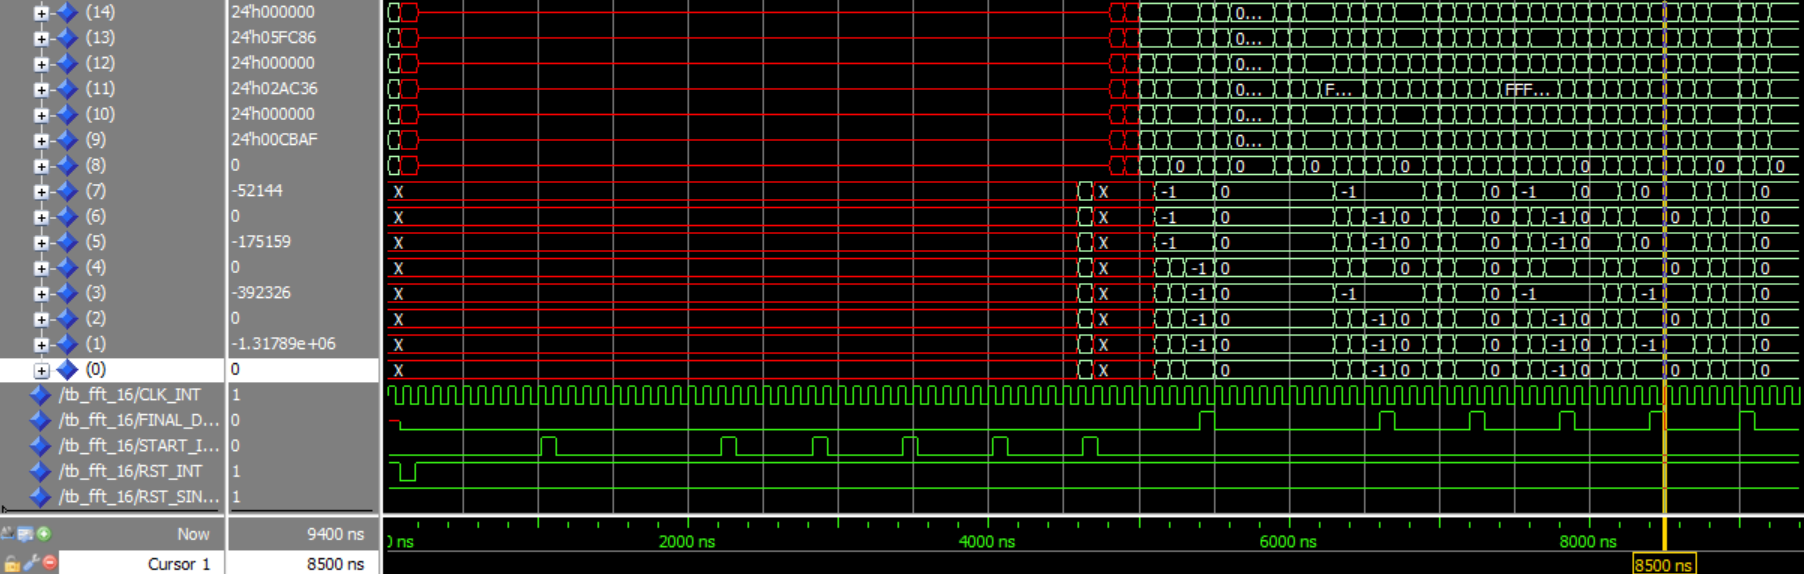
\includegraphics[width=1\textwidth]{sim_test5_imag}
      \caption{Schermata della simulazione completa, con focus sulle parti immaginarie dei risultati del test 5}
\end{figure}
\begin{figure}[H]
      \centering
      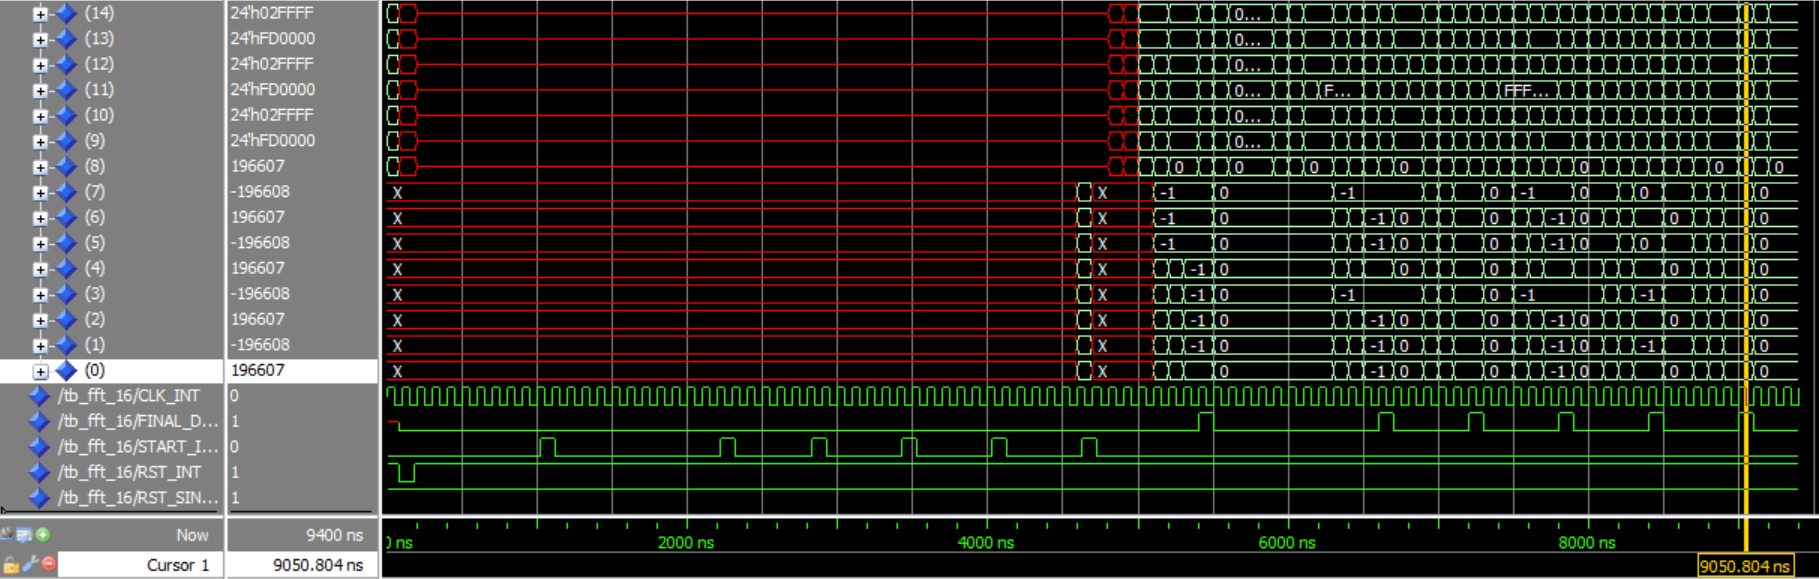
\includegraphics[width=1\textwidth]{sim_test6_real}
      \caption{Schermata della simulazione completa, con focus sulle parti reali dei risultati del test 6}
\end{figure}
\begin{figure}[H]
      \centering
      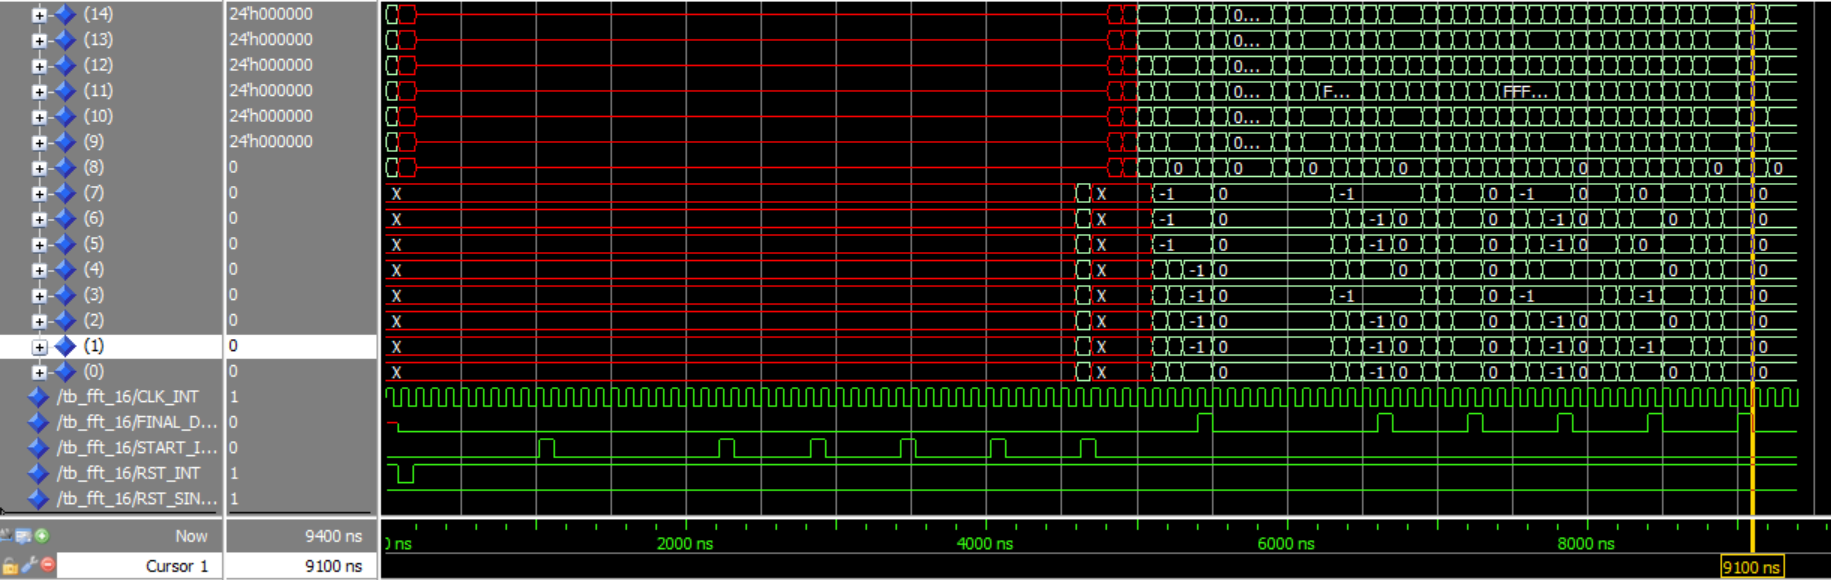
\includegraphics[width=1\textwidth]{sim_test6_imag}
      \caption{Schermata della simulazione completa, con focus sulle parti immaginarie dei risultati del test 6}
\end{figure}
\noindent Dalle schermate riportate della simulazione completa, in cui il periodo di clock è stato impostato a 100 ns, si sottolinea come gli output soddisfino i valori attesi dai sei test. Si osserva anche che il primo fronte di START avviene a 1100 ns e il relativo DONE (indicato come $FINAL\_DONE$) è alto in corrispondenza del fronte a 5500 ns. La differenza è esattamente 4400 ns, che è il tempo necessario per una butterfly a generare un segnale DONE (1100 ns rispetto al fronte di salita del clock in cui è attivo lo START relativo) moltiplicato per 4 (il numero di stadi). Perciò, come atteso, la latenza di una singola butterfly risulta essere pari a 12 periodi di clock (poi le parti immaginarie vengono fornite in uscita il colpo successivo all'attivazione del done), mentre la latenza di ogni FFT è di 45 colpi di clock. Inoltre, si osserva che, nonostante la latenza sia la medesima sia in modalità continua che in modalità singola, nel primo caso genero un segnale di DONE (e quindi risultati validi) ogni 6 colpi di clock.

\noindent A seguire, si riportano le tabelle in cui vengono confrontati i risultati aspettati con quelli ottenuti dalla simulazione, tenendo conto che, per rapportare correttamente i valori espressi come signed forniti in ambito simulativo con le uscite attese, è necessario convertirli in fixed point, dividendo per $2^{23}$, e moltiplicarli per lo scale factor, pari a 32. I dati ottenuti risultano essere estremamente precisi e in accordo con i risultati attesi, anche per via del ridotto numero di cifre significative dei risultati con cui si è effettuata la comparazione.

\begin{table}[H]
\centering
\resizebox{\textwidth}{!}{% % Forza la tabella a stare nella larghezza del testo
\begin{tabular}{|c|c|c|c|c|c|c|}
\hline
\textit{Indice} & \begin{tabular}[c]{@{}c@{}}\textit{parte reale}\\\textit{attesa}\end{tabular} & \begin{tabular}[c]{@{}c@{}}\textit{parte immaginaria}\\\textit{attesa}\end{tabular} & \begin{tabular}[c]{@{}c@{}}\textit{parte reale}\\\textit{da simulaz.}\end{tabular} & \begin{tabular}[c]{@{}c@{}}\textit{parte immaginaria}\\\textit{da simulaz.}\end{tabular} & \begin{tabular}[c]{@{}c@{}}\textit{parte reale}\\\textit{scalata}\end{tabular} & \begin{tabular}[c]{@{}c@{}}\textit{parte immaginaria}\\\textit{scalata}\end{tabular} \\ \hline
0 & -16 & 0 & -4.1943e+06 & 0 & $\approx$ -15.99998 & 0 \\ \hline
1 & 0 & 0 & -1 & 0 & $\approx$ -3.8e-06 & 0 \\ \hline
2 & 0 & 0 & -1 & 0 & $\approx$ -3.8e-06 & 0 \\ \hline
3 & 0 & 0 & -1 & 0 & $\approx$ -3.8e-06 & 0 \\ \hline
4 & 0 & 0 & -1 & 0 & $\approx$ -3.8e-06 & 0 \\ \hline
5 & 0 & 0 & -1 & 0 & $\approx$ -3.8e-06 & 0 \\ \hline
6 & 0 & 0 & -1 & 0 & $\approx$ -3.8e-06 & 0 \\ \hline
7 & 0 & 0 & -1 & 0 & $\approx$ -3.8e-06 & 0 \\ \hline
8 & 0 & 0 & -1 & 0 & $\approx$ -3.8e-06 & 0 \\ \hline
\end{tabular}%
}
\caption{Tabella riassuntiva per il vettore di test 1}
\end{table}

\begin{table}[H]
\centering
\resizebox{\textwidth}{!}{% % Adatta la tabella alla larghezza della pagina
\begin{tabular}{|c|c|c|c|c|c|c|}
\hline
\textit{Indice} & \begin{tabular}[c]{@{}c@{}}\textit{parte reale}\\\textit{attesa}\end{tabular} & \begin{tabular}[c]{@{}c@{}}\textit{parte immaginaria}\\\textit{attesa}\end{tabular} & \begin{tabular}[c]{@{}c@{}}\textit{parte reale}\\\textit{da simulaz.}\end{tabular} & \begin{tabular}[c]{@{}c@{}}\textit{parte immaginaria}\\\textit{da simulaz.}\end{tabular} & \begin{tabular}[c]{@{}c@{}}\textit{parte reale}\\\textit{scalata}\end{tabular} & \begin{tabular}[c]{@{}c@{}}\textit{parte immaginaria}\\\textit{scalata}\end{tabular} \\ \hline
0 & 0 & 0 & -1 & 0 & $\approx$ -3.8e-06 & 0 \\ \hline
1 & 0 & 0 & -1 & 0 & $\approx$ -3.8e-06 & 0 \\ \hline
2 & 0 & 0 & -1 & 0 & $\approx$ -3.8e-06 & 0 \\ \hline
3 & 0 & 0 & -1 & -1 & $\approx$ -3.8e-06 & $\approx$ -3.8e-06  \\ \hline
4 & -8 & 0 & -2.09715e+06 & 0 & $\approx$ -7.999992 & 0 \\ \hline
5 & 0 & 0 & -1 & 0 & $\approx$ -3.8e-06 & 0 \\ \hline
6 & 0 & 0 & -1 & 0 & $\approx$ -3.8e-06 & 0 \\ \hline
7 & 0 & 0 & -1 & -1 & $\approx$ -3.8e-06 & $\approx$ -3.8e-06  \\ \hline
8 & 0 & 0 & -1 & 0 & $\approx$ -3.8e-06 & 0 \\ \hline
\end{tabular}%
}
\caption{Tabella riassuntiva per il vettore di test 2}
\end{table}

\begin{table}[H]
\centering
\resizebox{\textwidth}{!}{% % Adatta la tabella alla larghezza della pagina
\begin{tabular}{|c|c|c|c|c|c|c|}
\hline
\textit{Indice} & \begin{tabular}[c]{@{}c@{}}\textit{parte reale}\\\textit{attesa}\end{tabular} & \begin{tabular}[c]{@{}c@{}}\textit{parte immaginaria}\\\textit{attesa}\end{tabular} & \begin{tabular}[c]{@{}c@{}}\textit{parte reale}\\\textit{da simulaz.}\end{tabular} & \begin{tabular}[c]{@{}c@{}}\textit{parte immaginaria}\\\textit{da simulaz.}\end{tabular} & \begin{tabular}[c]{@{}c@{}}\textit{parte reale}\\\textit{scalata}\end{tabular} & \begin{tabular}[c]{@{}c@{}}\textit{parte immaginaria}\\\textit{scalata}\end{tabular} \\ \hline
0 & 1 & 0 & 262143 & 0 & $\approx$ 0.999996 & 0 \\ \hline
1 & 1 & 0 & 262143 & 0 & $\approx$ 0.999996 & 0 \\ \hline
2 & 1 & 0 & 262143 & 0 & $\approx$ 0.999996 & 0 \\ \hline
3 & 1 & 0 & 262143 & 0 & $\approx$ 0.999996 & 0 \\ \hline
4 & 1 & 0 & 262143 & 0 & $\approx$ 0.999996 & 0 \\ \hline
5 & 1 & 0 & 262143 & 0 & $\approx$ 0.999996 & 0 \\ \hline
6 & 1 & 0 & 262143 & 0 & $\approx$ 0.999996 & 0 \\ \hline
7 & 1 & 0 & 262143 & 0 & $\approx$ 0.999996 & 0 \\ \hline
8 & 1 & 0 & 262143 & 0 & $\approx$ 0.999996 & 0 \\ \hline
\end{tabular}%
}
\caption{Tabella riassuntiva per il vettore di test 3}
\end{table}

\begin{table}[H]
\centering
\resizebox{\textwidth}{!}{% % Adatta la tabella alla larghezza della pagina
\begin{tabular}{|c|c|c|c|c|c|c|}
\hline
\textit{Indice} & \begin{tabular}[c]{@{}c@{}}\textit{parte reale}\\\textit{attesa}\end{tabular} & \begin{tabular}[c]{@{}c@{}}\textit{parte immaginaria}\\\textit{attesa}\end{tabular} & \begin{tabular}[c]{@{}c@{}}\textit{parte reale}\\\textit{da simulaz.}\end{tabular} & \begin{tabular}[c]{@{}c@{}}\textit{parte immaginaria}\\\textit{da simulaz.}\end{tabular} & \begin{tabular}[c]{@{}c@{}}\textit{parte reale}\\\textit{scalata}\end{tabular} & \begin{tabular}[c]{@{}c@{}}\textit{parte immaginaria}\\\textit{scalata}\end{tabular} \\ \hline
0 & 0 & 0 & -1 & 0 & $\approx$ -3.8e-06 & 0 \\ \hline
1 & 0 & 0 & -1 & 0 & $\approx$ -3.8e-06 & 0 \\ \hline
2 & 0 & 0 & -1 & 0 & $\approx$ -3.8e-06 & 0 \\ \hline
3 & 0 & 0 & -1 & -1 & $\approx$ -3.8e-06 & $\approx$ -3.8e-06 \\ \hline
4 & -8 & 8 & -2.09715e+06 & 2.09715e+06 & $\approx$ -7.999992 & $\approx$ +7.999992 \\ \hline
5 & 0 & 0 & -1 & 0 & $\approx$ -3.8e-06 & 0 \\ \hline
6 & 0 & 0 & -1 & 0 & $\approx$ -3.8e-06 & 0 \\ \hline
7 & 0 & 0 & -1 & 0 & $\approx$ -3.8e-06 & 0 \\ \hline
8 & 0 & 0 & -1 & 0 & $\approx$ -3.8e-06 & 0 \\ \hline
\end{tabular}%
}
\caption{Tabella riassuntiva per il vettore di test 4}
\end{table}

\begin{table}[H]
\centering
\resizebox{\textwidth}{!}{% % Adatta la tabella alla larghezza della pagina
\begin{tabular}{|c|c|c|c|c|c|c|}
\hline
\textit{Indice} & \begin{tabular}[c]{@{}c@{}}\textit{parte reale}\\\textit{attesa}\end{tabular} & \begin{tabular}[c]{@{}c@{}}\textit{parte immaginaria}\\\textit{attesa}\end{tabular} & \begin{tabular}[c]{@{}c@{}}\textit{parte reale}\\\textit{da simulaz.}\end{tabular} & \begin{tabular}[c]{@{}c@{}}\textit{parte immaginaria}\\\textit{da simulaz.}\end{tabular} & \begin{tabular}[c]{@{}c@{}}\textit{parte reale}\\\textit{scalata}\end{tabular} & \begin{tabular}[c]{@{}c@{}}\textit{parte immaginaria}\\\textit{scalata}\end{tabular} \\ \hline
0 & 1 & 0 & 262143 & 0 & $\approx$ 0.999996 & 0 \\ \hline
1 & 0 & -5.027 & -1 & -1.31789e+06 & $\approx$ -3.8e-06 & $\approx$ -5.027 \\ \hline
2 & 1 & 0 & 262143 & 0 & $\approx$ 0.999996 & 0 \\ \hline
3 & 0 & -1.497 & -1 & -392326 & $\approx$ -3.8e-06 & $\approx$ -1.497 \\ \hline
4 & 1 & 0 & 262143 & 0 & $\approx$ 0.999996 & 0 \\ \hline
5 & 0 & -0.668 & 0 & -175159 & 0 & $\approx$ -0.668 \\ \hline
6 & 1 & 0 & 262143 & 0 & $\approx$ 0.999996 & 0 \\ \hline
7 & 0 & -0.199 & 0 & -52144 & 0 & $\approx$ -0.199 \\ \hline
8 & 1 & 0 & 262143 & 0 & $\approx$ 0.999996 & 0 \\ \hline
\end{tabular}%
}
\caption{Tabella riassuntiva per il vettore di test 5}
\end{table}


\begin{table}[H]
\centering
\resizebox{\textwidth}{!}{% % Adatta la tabella alla larghezza della pagina
\begin{tabular}{|c|c|c|c|c|c|c|}
\hline
\textit{Indice} & \begin{tabular}[c]{@{}c@{}}\textit{parte reale}\\\textit{attesa}\end{tabular} & \begin{tabular}[c]{@{}c@{}}\textit{parte immaginaria}\\\textit{attesa}\end{tabular} & \begin{tabular}[c]{@{}c@{}}\textit{parte reale}\\\textit{da simulaz.}\end{tabular} & \begin{tabular}[c]{@{}c@{}}\textit{parte immaginaria}\\\textit{da simulaz.}\end{tabular} & \begin{tabular}[c]{@{}c@{}}\textit{parte reale}\\\textit{scalata}\end{tabular} & \begin{tabular}[c]{@{}c@{}}\textit{parte immaginaria}\\\textit{scalata}\end{tabular} \\ \hline
0 & 0.75 & 0 & 196607 & 0 & $\approx$ 0.749996 & 0 \\ \hline
1 & -0.75 & 0 & -196608 & 0 &  -0.75 & 0 \\ \hline
2 & 0.75 & 0 & 196607 & 0 & $\approx$ 0.749996 & 0 \\ \hline
3 & -0.75 & 0 & -196608 & 0 &  -0.75 & 0 \\ \hline
4 & 0.75 & 0 & 196607 & 0 & $\approx$ 0.749996 & 0 \\ \hline
5 & -0.75 & 0 & -196608 & 0 &  -0.75 & 0 \\ \hline
6 & 0.75 & 0 & 196607 & 0 & $\approx$ 0.749996 & 0 \\ \hline
7 & -0.75 & 0 & -196608 & 0 &  -0.75 & 0 \\ \hline
8 & 0.75 & 0 & 196607 & 0 & $\approx$ 0.749996 & 0 \\ \hline
\end{tabular}%
}
\caption{Tabella riassuntiva per il vettore di test 6}
\end{table}


\noindent Infine, si riporta lo screenshot di una simulazione dedicata, che mostra l'effetto del Reset Sincrono (indicato come RST\_SINC\_INT); successivamente all'attivazione di tale segnale, come descritto nella sottosezione \ref{subsec:reset}, tutte le butterfly presenti nell'architettura vengono riportate allo stato di IDLE. Infatti,  è possibile notare come, nonostante siano stati inviati correttamente 7 segnali di START, si trasmettono in uscita dalla FFT solo cinque segnali di DONE attivi; poiché la terza e la quarta elaborazione richiesta dei dati in ingresso non è ancora terminata quando viene richiesto un reset della macchina.


\begin{figure}[H]
      \centering
      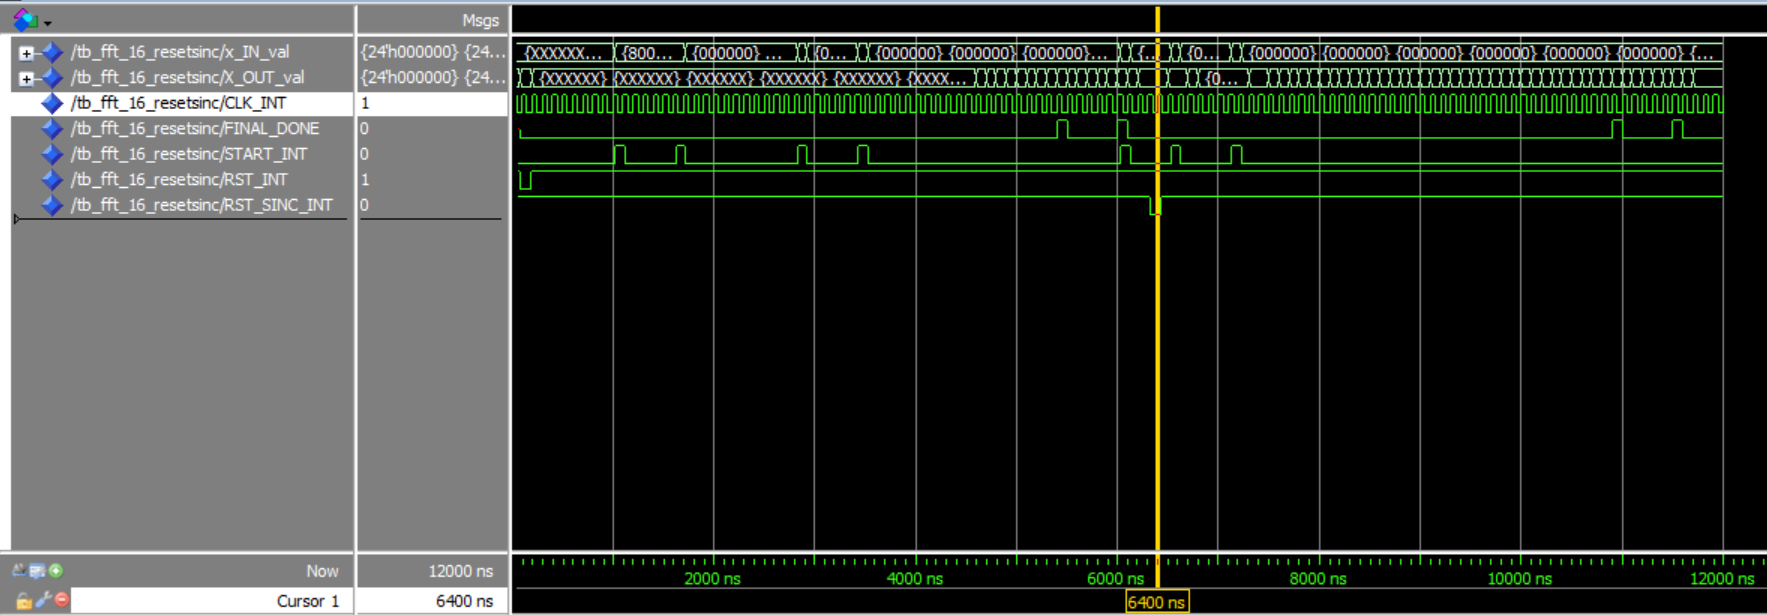
\includegraphics[width=1\textwidth]{sim_reset_sinc}
      \caption{Schermata della simulazione completa, con focus sul Reset Sincrono}
\end{figure}

\section{Sviluppi Futuri}
Per ragioni progettuali, di tempo e date le forti limitazioni, sono rimasti alcuni punti che potrebbero essere modificati con lo scopo di migliorare la stabilità e il rendimento del progetto.

\begin{itemize}
\item   Reset asincrono: Data la specifica, per la quale non si potevano inserire componenti all’esterno delle Butterfly,  abbiamo una connessione che risulta diretta con l’esterno e quindi condizionata dal rumore. La presenza di glitch rischierebbe quindi di resettare la macchina perdendo il lavoro in esecuzione. Questo problema può essere risolto con il campionamento di suddetto ingresso o anche solo con un controllo della durata del reset con lo scopo di evitare che brevissimi glitch influenzino la macchina a stati (una porta AND fra il segnale di reset e il segnale di reset ritardato tramite 2$\cdot$N inverter in cascata, il cui numero è da stabilire in base alla tecnologia).
\item   Gestione dei W : Siamo consapevoli che la soluzione meno costosa e più efficace è sicuramente quella di porre i pin di ingresso per ogni singola Butterfly ai suoi $W_r$ e $W_i$ dedicati, ma questo può limitare la flessibilità del progetto e, in caso di errore nella realizzazione dei valori inchiodati, potrebbe rendere inutilizzabile il circuito. Perciò, se servisse maggiore flessibilità nell'invio dei W, si è quindi pensato a un sistema basato sul passaggio dei W attraverso un Bus e un enable codificato per la selezione dei riceventi. Questa soluzione però è soddisfacente fino al caso con 32 campioni, dato che con 64 campioni (per cui servono 6 colonne da 32 Butterfly) si avrebbero 32 W da passare per un totale di 64 valori che vanno consegnati entro lo start dell’ultima colonna che avviene al 55-esimo colpo (T\_ Butterfly * (N\_colonne -1)=11*5=55).
\item Uscite: per limitare il rumore e i consumi prodotti dalle uscite delle singole Butterfly si potrebbe introdurre una porta AND per ogni uscita, che fa passare l’uscita solo quando si sta trasmettendo un segnale DONE e al colpo ad esso successivo (salvando questa informazione in un FF).
\end{itemize}

\section{Conclusioni}
Alla luce dei test svolti e delle spiegazioni fornite possiamo sostenere di aver centrato il goal prefissato dato il throughput raggiunto in continua e la precisione ottenuta.
Riassumendo il lavoro svolto: abbiamo progettato un elaboratore che risolve la fft su 16 campioni attraverso l’uso di 32 (8x4) Butterfly, componente microprogrammato che implementa la tecnica dei Late Status, ottenendo una latenza di 45 colpi di clock tra il momento in cui si ha uno start in corrispondenza di un rising edge del clk e l’output delle parti immaginarie e un throughput pari a una solve ogni 6 colpi di clock in modalità continua.


\end{document}
